%%%%%%%%%%%%%%%%%%%%%%%%%%%%%%%%%%%%%%%%%%%%%%%%%%%%%%%%%%%%%%%%%%%%%
%%                                                                 %%
%% Please do not use \input{...} to include other tex files.       %%
%% Submit your LaTeX manuscript as one .tex document.              %%
%%                                                                 %%
%% All additional figures and files should be attached             %%
%% separately and not embedded in the \TeX\ document itself.       %%
%%                                                                 %%
%%%%%%%%%%%%%%%%%%%%%%%%%%%%%%%%%%%%%%%%%%%%%%%%%%%%%%%%%%%%%%%%%%%%%

%%\documentclass[referee,sn-basic]{sn-jnl}% referee option is meant for double line spacing

%%=======================================================%%
%% to print line numbers in the margin use lineno option %%
%%=======================================================%%

%%\documentclass[lineno,sn-basic]{sn-jnl}% Basic Springer Nature Reference Style/Chemistry Reference Style

%%======================================================%%
%% to compile with pdflatex/xelatex use pdflatex option %%
%%======================================================%%

%%\documentclass[pdflatex,sn-basic]{sn-jnl}% Basic Springer Nature Reference Style/Chemistry Reference Style

%%\documentclass[sn-basic]{sn-jnl}% Basic Springer Nature Reference Style/Chemistry Reference Style
\documentclass[sn-mathphys,Numbered]{sn-jnl}% Math and Physical Sciences Reference Style
%%\documentclass[sn-aps]{sn-jnl}% American Physical Society (APS) Reference Style
%%\documentclass[sn-vancouver]{sn-jnl}% Vancouver Reference Style
%%\documentclass[sn-apa]{sn-jnl}% APA Reference Style
%%\documentclass[sn-chicago]{sn-jnl}% Chicago-based Humanities Reference Style
%%\documentclass[sn-standardnature]{sn-jnl}% Standard Nature Portfolio Reference Style
%%\documentclass[default]{sn-jnl}% Default
%%\documentclass[default,iicol]{sn-jnl}% Default with double column layout

%%%% Standard Packages
%%<additional latex packages if required can be included here>
%%%%

%%%%%=============================================================================%%%%
%%%%  Remarks: This template is provided to aid authors with the preparation
%%%%  of original research articles intended for submission to journals published 
%%%%  by Springer Nature. The guidance has been prepared in partnership with 
%%%%  production teams to conform to Springer Nature technical requirements. 
%%%%  Editorial and presentation requirements differ among journal portfolios and 
%%%%  research disciplines. You may find sections in this template are irrelevant 
%%%%  to your work and are empowered to omit any such section if allowed by the 
%%%%  journal you intend to submit to. The submission guidelines and policies 
%%%%  of the journal take precedence. A detailed User Manual is available in the 
%%%%  template package for technical guidance.
%%%%%=============================================================================%%%%

\jyear{2021}%

%% as per the requirement new theorem styles can be included as shown below
\theoremstyle{thmstyleone}%
\newtheorem{theorem}{Theorem}%  meant for continuous numbers
%%\newtheorem{theorem}{Theorem}[section]% meant for sectionwise numbers
%% optional argument [theorem] produces theorem numbering sequence instead of independent numbers for Proposition
\newtheorem{proposition}[theorem]{Proposition}% 
%%\newtheorem{proposition}{Proposition}% to get separate numbers for theorem and proposition etc.

\theoremstyle{thmstyletwo}%
\newtheorem{example}{Example}%
\newtheorem{remark}{Remark}%

\theoremstyle{thmstylethree}%
\newtheorem{definition}{Definition}%

\raggedbottom
%%\unnumbered% uncomment this for unnumbered level heads

%% My used library
\usepackage{subcaption}
\usepackage{amsmath,amssymb}
\usepackage{graphicx, adjustbox}
\usepackage{caption}
\usepackage{longtable,booktabs,array}
\usepackage{csquotes}
\graphicspath{{Figs}{Figs/}}

\begin{document}

\title[Article Title]{Unsupervised Topic Modeling with LDA for Textbook Content Comprehension,
a qualitative survey}

%%=============================================================%%
%% Prefix	-> \pfx{Dr}
%% GivenName	-> \fnm{Joergen W.}
%% Particle	-> \spfx{van der} -> surname prefix
%% FamilyName	-> \sur{Ploeg}
%% Suffix	-> \sfx{IV}
%% NatureName	-> \tanm{Poet Laureate} -> Title after name
%% Degrees	-> \dgr{MSc, PhD}
%% \author*[1,2]{\pfx{Dr} \fnm{Joergen W.} \spfx{van der} \sur{Ploeg} \sfx{IV} \tanm{Poet Laureate} 
%%                 \dgr{MSc, PhD}}\email{iauthor@gmail.com}
%%=============================================================%%

\author*[1,2]{\fnm{Md Iftekharul} \sur{Mobin}}\email{iftekhar.mobin@gmail.com}

\author[2,3]{\fnm{Second} \sur{Author}}\email{iiauthor@gmail.com}
\equalcont{These authors contributed equally to this work.}

\author[1,2]{\fnm{Third} \sur{Author}}\email{iiiauthor@gmail.com}
\equalcont{These authors contributed equally to this work.}

\affil*[1]{\orgdiv{Department}, \orgname{Organization}, \orgaddress{\street{Street}, \city{City}, \postcode{100190}, \state{State}, \country{Country}}}

\affil[2]{\orgdiv{Department}, \orgname{Organization}, \orgaddress{\street{Street}, \city{City}, \postcode{10587}, \state{State}, \country{Country}}}

\affil[3]{\orgdiv{Department}, \orgname{Organization}, \orgaddress{\street{Street}, \city{City}, \postcode{610101}, \state{State}, \country{Country}}}

%%==================================%%
%% sample for unstructured abstract %%
%%==================================%%

\abstract{In this research LDA driven exploratory analysis is shown to depict
various keywords related to subtle topic in context. It identifies
latent topics within textbook lessons, uncovers coherent themes from
textual data, aims to improve the curriculum provided English textbook
content synthesis and acquisition skill of learners. It is anticipated
extracted topics enable readers to comprehend the curriculum material
more efficiently. Extensive analysis is conducted to visualize, high
impact keywords, co-occurrence patterns and correlation between extracted
topics. A prototype mobile app is developed which incorporates topic
modeling extracted keywords. Furthermore, qualitative research survey is
undertaken to evaluate its effectiveness on end-users (course
instructors of Bangladesh\textquotesingle s higher secondary school). The
challenges, future potential of LDA extracted content integrated mobile
app into the learning process is explored. After collecting feedback,
word clouds were used to analyze the participants\textquotesingle{}
recommended terms, and the LIWC approach is used to estimate overall
sentiment. LIWC score showed positive sentiment and survey process
enticed the participants, demonstrates learners eager to use NLP
technology driven topic modeling approach in teaching and learning, and
there are tremendous opportunities.}



%%================================%%
%% Sample for structured abstract %%
%%================================%%

% \abstract{\textbf{Purpose:} The abstract serves both as a general introduction to the topic and as a brief, non-technical summary of the main results and their implications. The abstract must not include subheadings (unless expressly permitted in the journal's Instructions to Authors), equations or citations. As a guide the abstract should not exceed 200 words. Most journals do not set a hard limit however authors are advised to check the author instructions for the journal they are submitting to.
% 
% \textbf{Methods:} The abstract serves both as a general introduction to the topic and as a brief, non-technical summary of the main results and their implications. The abstract must not include subheadings (unless expressly permitted in the journal's Instructions to Authors), equations or citations. As a guide the abstract should not exceed 200 words. Most journals do not set a hard limit however authors are advised to check the author instructions for the journal they are submitting to.
% 
% \textbf{Results:} The abstract serves both as a general introduction to the topic and as a brief, non-technical summary of the main results and their implications. The abstract must not include subheadings (unless expressly permitted in the journal's Instructions to Authors), equations or citations. As a guide the abstract should not exceed 200 words. Most journals do not set a hard limit however authors are advised to check the author instructions for the journal they are submitting to.
% 
% \textbf{Conclusion:} The abstract serves both as a general introduction to the topic and as a brief, non-technical summary of the main results and their implications. The abstract must not include subheadings (unless expressly permitted in the journal's Instructions to Authors), equations or citations. As a guide the abstract should not exceed 200 words. Most journals do not set a hard limit however authors are advised to check the author instructions for the journal they are submitting to.}

\keywords{Natural Language Processing (NLP), Topic Modeling, Latent Dirichlet Allocation (LDA), Exploratory Analysis, Textbook Learning, Coherence}

%%\pacs[JEL Classification]{D8, H51}

%%\pacs[MSC Classification]{35A01, 65L10, 65L12, 65L20, 65L70}

\maketitle

\section{Introduction}\label{sec1}
In Bangladesh there is lacking in effective acquisition, synthesis skill of English language from National Curriculum and Textbook Board (NCTB) curriculum provided textbook {[}1{]}--{[}4{]}. Specially in the rural area in National Board examinations like SSC, HSC most of the student get poor marks in English subject. It is anticipated students have lacking in understanding context. Topic modeling can play a significant role for context understanding for curriculum provided English textbook. Topic modeling is machine learning technique of Natural Language Processing field, offers a promising unsupervised approach to identify latent topics within provided documents. It can help identify the main themes, concepts, and topics within the textbook\textquotesingle s content, enabling instructors to tailor the learning experience to individual students. LDA is one the prominent algorithm which can be used for topic modeling. It provides coherent topics, dominant keywords, latent combination of features that characterizes similarities between topics. In this research LDA extracted keywords are rearranged and incorporated into a mobile app to observe user experience. Some renowned mobile apps are Duolingo, Busuu, Babel, Voxy etc {[}25{]}. Across all English learning applications via digital media, 55\% have activities for vocabulary learning and other exercises are about 41\% {[}18{]}, {[}19{]} includes quizzes, exercises, and game for enhancing learners' comprehension and self-checks {[}17{]}. One caveat is of these apps are these are not based on Curriculum Board provided Textbook for learning English hence, could not able to attract a large number of pupils in Bangladesh who are mostly depended on NCBI textbook.  To grasp the English language knowledge from curriculum provided textbook a novel approach LDA based unsupervised Topic modeling using textbook corpus is adopted and exploratory analysis is demonstrated in this study. Our anticipation is through this way student can able to interpret meaningful information facilitates students to understand the correlated topics and important keywords related to that topics leads to understand the subtle meaning of the textbook context.

\subsection{Research Overview} 
To detect underlying themes or topics keywords within a Textbook corpus an unsupervised probabilistic topic modeling technique Latent Dirichlet Allocation (LDA) is used in this research. Topic modeling of LDA doesn\textquotesingle t directly account for student engagement such as learning tasks in mobile apps. Hence a prototype app is developed and qualitative survey is conducted to observe the instructor\textquotesingle s sentiment impact. Qualitative survey research is undertaken to evaluate the effectiveness of unsupervised topic modeling LDA Bangladesh\textquotesingle s National Curriculum Textbook Board (NCTB) provided English Textbook for Higher secondary school education. This study seeks to ascertain if students can learn English better if a mobile app is introduced which includes NLP\textquotesingle s LDA driven topic modeling applied extracted keywords and analysis. A prototype mobile app is developed to incorporate the topic modeling extracted keywords into the app. This article presents the key findings and insights from the survey, shedding light on the prospective of learners especially instructors. In the survey questions, it was indicated whether the students, teachers/instructors, and government organizations would find it acceptable and appreciated if textbook information were made available through a mobile app and presented in interactive format. To demonstrate the mobile app idea during the interrogation survey session a prototype is also prepared. Participants were asked for suggestions on how to make the app better and about any shortcomings. After collecting feedback, word clouds were used to analyze the frequency of the participants\textquotesingle{} recommended terms, and the LIWC approach was used to estimate overall sentiment. The survey\textquotesingle s findings show that teachers are eager to use NLP provided extracted keywords technology in teaching and learning, and there are tremendous opportunities.

\subsection{Topic Modeling}
 Different techniques have been developed to perform topic modeling in the unsupervised topic modeling domain of Natural Language Processing (NLP), having their own strengths and limitations. Apart from LDA, Mallet LDA, Structural Topic Model (STM), Hierarchical Dirichlet Process (HDP), Non-Negative Matrix Factorization (NMF), Latent Semantic Analysis (LSA) etc are also prevailing and can be considered for comparative research study.

\subsubsection{Topic models comparative analysis}
While some variations of LDA, Mallet LDA is considered for large corpus processing and analysis. It focuses on scalability, If large corpus needs to analyze, Mallet LDA might be more suitable. LDA in general can still be efficiently applied to moderately sized corpora. Analyzing topics within the context of metadata, STM could be a better fit. Hierarchical Dirichlet Process (HDP) can be useful when we cannot guess the number of topics in advance. However, as a baseline model LDA is often considered one of the most prominent choices. In this study Textbook corpus is divided into lessons which is a mixture of topics and using LDA expecting to determine which word in the lesson belong to Lesson\textquotesingle s topics. LDA produces interpretative results for exploratory topic analysis. The identified topics are represented as distributions over words, making it easy to assign meaningful labels to topics. Provided by most of the libraries and tools, making it easy to implement and can be integrated into existing workflows. Hence, LDA serves as a solid baseline for topic modeling tasks. 

\section{Latent Dirichlet Allocation (LDA)}
LDA model considers documents are mixes of topic, and each topic is a distribution over words. The objective is to derive the hidden topic assignments and the topic-word distributions that most effectively describe the observed documents. The goal of LDA is to uncover these latent topics from a collection of documents without needing any prior labeling or categorization of the content. An expression for the joint distribution of the LDA model is described below:  
\begin{equation}
P(\theta_d,z,w\|\alpha,\beta)=P(\theta_d\|\alpha)\prod^N_{n=1}P(z_{d,n}\|\theta_d)P(w_{d,n}\|z_{d,n},\beta)
\end{equation}
Where $w_{d,n}$ the $n_{th}$ word in document $d$, $z_{d,n}$ the topic assigned to the $n_{th}$ word in document $d$, $\alpha,\beta$ are the Dirichlet LDA model parameters. controls per-document topic distribution, and per topic word distribution. $\theta_d$ represent the topic distribution. $P(\theta_d \| \alpha)$ Dirichlet 
distribution representing the document-topic distribution, $P(z_{d,n}\|\theta_d)$ is the word topic assignment for the $n_{th}$ word in document $d$, $P(w_{d,n}\|z_{d,n},\beta)$ is the distribution representing the observed word given a topic. We have chosen LDA for baseline statistical topic modeling tool. However, how many topics are ideal it is needed to determine and also topic modeling quality needs to measure.


\subsection{Optimal Topics with Coherence}  
Coherence score measure how coherent or interpret the words in that topic and estimates number of topic clusters. Coherence score assess the quality of the topics produced by LDA and ensures that the topics generated are statistically significant. Coherence \(C_{topic}\) can be expressed as follows  
\begin{equation}
C_{topic}=\sum^N_{i=1} (\frac{1}{N(N-1)}\sum^i_{j=1} PMI(w_i,w_j)
\end{equation}
Where, \(PMI\left( w_{i},w_{j} \right)\) represent pointwise mutual information statistical association between two words occurring together. PMI score indicates that the two words are more closely related within a topic. \(PMI\left( w_{i},w_{j} \right)\) can expressed as  
\begin{equation}
\(PMI\left( w_{i},w_{j} \right) = \log\frac{P\left( w_{i},w_{j} \right)}{P\left( w_{i} \right)P\left( w_{j} \right)}\)
\end{equation}

where \(P\left( w_{i},w_{j} \right)\) is joint probability of occurrence of words \(w_{i}\) and \(w_{j}\).  To calculate the coherence score genism library provides range of options such as \(u_{mass},c_{v},c_{uci},c_{npmi}\). \(u_{mass}\) and \(c_{v}\)These two methods are most popular. For given topic with words \(\{ w_{1},w_{2},w_{3},\ldots..,w_{n}\}\) a fixed context window size is provided (default size 10 words) then coherence score is calculated using an equation \(\sum_{j = 1}^{i}{PMI}\left( w_{i},w_{j} \right)\) which provides negative coherence score. \(c_{v}\) can be expressed as  
\begin{equation}
\(c_{v} = \frac{1}{N(N - 1)}\sum_{j = 1}^{i}{similarity\left( w_{i},w_{j} \right)}\)
\end{equation}
in which \(similarity\left( w_{i},w_{j} \right)\) represent the pairwise similarity between terms based on \(PMI\left( w_{i},w_{j} \right)\) scores. \(c_{v}\) provides a positive coherence score. Higher coherence values indicate that the topics are more coherent and representative of meaningful themes within the text data. Coherence score 0.5 are fairly good {[}43{]}.
  
\section{Literature Review}

LDA based topic modeling has been used for semantic search, ontology exploration, classification, dominant keywords searching in many research studies. For curriculum based textbook study it could be an option is not revealed from rigorous search in online repositories, which we addressed in this research study. This research model is infusing Textbook features into LDA based topic modeling to discover a set of topic-words from the provided document for Textbook comprehension and understanding context. Similar approaches and implications are described below:

\subsection{LDA for Textbook Content}

According to Krishna Raj {[}41{]} the human brain has a propensity to forget a number of facts regarding the events in book. The LDA model can able to scan through large quantities of text in the book and extract intriguing key concepts terms. Thereby, a book can be adapted by learners with the help of the LDA model, greatly refine the learning process. Similar approch proposed by  Rani For Hindi books and stories, a topic modeling text summarizing approach proposed in 2020 {[}42{]}. By incorporating linguistic features into LDA-based topic modeling, the suggested model is can find a set of topic-words from the given material to understand context.  Educational content-based topic modeling for an Intelligent system to develop a tutoring system is proposed in {[}34{]} by researcher Stefan Slater in 2017. To understand the linguistic content of mathematical problems, a personalized learning system is suggested that makes use of correlated topic modeling of natural language processing, an approach which can extract important keywords. A variety of significant and useful contents are explored in the context of addressing mathematical difficulties. They demonstrated that topic modeling is a useful method for a personalized learning systems. For key terms detection within articles LDA based topic modeling has been used in many research studies in which dominant keywords reveals future research trends or most prominent topics. Investigation of Julio Guerra in 2013 demonstrated how the LDA model can be utilized for online content linking for any major subject such as: elementary algebra. It can also be used to simplify context comprehension and content modeling for collections of reference books on the same topic {[}33{]}. They concluded that the recommendation provided by LDA topic modeling for online educational systems is promising.
\subsection{LDA for Dominant Keywords Determination}

In 2019 Wafa Shafqat {[}38{]} proposed an architecture model for better understanding of crowdfunding comments posted by the investors to understand their motive to classify whether comments are scam or legitimate comments. Deep neural network Language modeling either LSTM or RNN encoded embedding vectors are fed into a LDA based topic modeling model to understand the context of discussion trends. Compared to simple Neural Networks (NNs) and non LDA based approach this techniques performs better understanding crowdfunding comments. The capability of LDA-based topic modeling to detect the reseach trend of Bengali news published in web was analyzed by Kazi Masudul Alam in 2020 {[}35{]}. Their research demonstrates that using an appropriate corpus and labeled LDA is an effective combination model for predicting news topics efficiently. LDA Labels key terms makes articles easier to read. Another research article of J. Lee published in 2022 conducted experiment on research trends of "COVID-19 and sports {[}36{]}. It used LDA and explored latent knowledge connectivity dimension and structures in the articles. Rahul Gupta {[}37{]} uses the application of LDA in 2022 to analyze research patterns of "Applied Intelligence" in 3269 articles published between 1991 to 2021. In this research BoW and TF-IDF embedding are used for LDA based topic modeling.

\subsection{LDA based Sentiment Analysis}

Sentiment analysis has been a key research area of NLP based research domain, where LDA has been applied to determine significant features and those features contributes to segregate sentiments and provide recommendations. LDA based topic modeling has been used in sentiment analysis task. In 2021 Y. Cho published research study of LDA-based topic modeling for sentiment analysis using topic/document/sentence (TDS) model {[}39{]}. This article proposed TDS novel approach that combines LDA-based topic modeling for sentiment analysis within documents. H. Wang and et. al examined Chinese people's public perception about Omicron variants on social media Sina Weibo. Social Media's 121,632 omicron related data post were analyzed using LDA-based topic modeling and sentiment analysis {[}40{]}. From topic analysis they realized omicron\textquotesingle s impact, infection situation, pandemic prevention and control geographically. Hence, it is actually revealed LDA based topic modeling can be used for understanding subtle topics and exploring various facts. Hence, from the above literature review we can infer LDA could help analyze the content of the textbook and identify the main topics covered. This information could then be used to enhance the learning experience.

\section{Methodology}
The methodology involves pre-processing textual data, training the LDA model on the pre-processed text, and subsequently interpreting and visualizing the generated topics. Data is collected from NCBI's English Textbook for class 9 of higher secondary school. Data mining approach is applied to segregate into subsequent lessons. Then textual data is pre-processed to remove noise, text standardizing, followed by the application of LDA to identify underlying topics, then coherence measurements are applied. Research overview is depicted as follows. 
\begin{adjustbox}{center, nofloat=figure, vspace=\bigskipamount, caption={Research workflow diagram}, label{fig:methodology_diagram}}
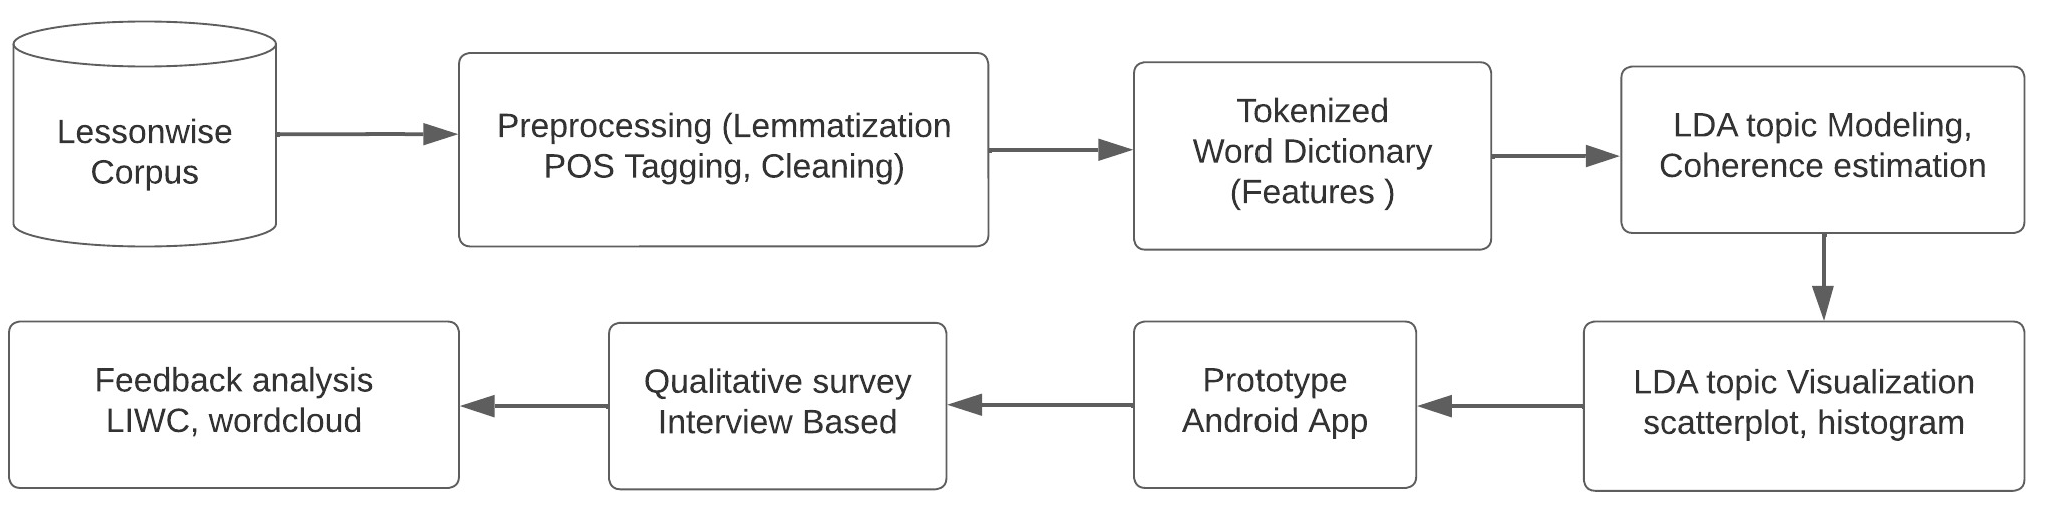
\includegraphics[width=0.9\textwidth]{Figs/methodology.png}
\end{adjustbox}

LDA algorithm automatically discovers latent topics within the documents based on word co-occurrences. Each topic will be represented by a set of words. Interpret these words to understand the main concepts associated with each topic. Extensive exploratory analysis is conducted to visualize the topic modeling outputs. Analyze the topics generated by the model require manual review and adjustment to ensure the topics make sense.

\section{Data Processing and Feature Extraction}

\begin{enumerate}
\def\labelenumi{\alph{enumi}.}
\item
  First NLP's data processing or data mining techniques are applied for meaningful token or feature extraction. Text is converted to Lowercased and Normalized to ensure consistent pre-processing.

  \begin{enumerate}
  \def\labelenumii{\roman{enumii}.}
  \item
    \textbf{Data cleaning}: unwanted characters, punctuation and special
    character removed and stop words (such as "and," "the," "is," etc)
    are removed. Spacy library's English word model and NLTK's stopwords
    list are used together. Also, words less than two characters are
    removed such as: I, Hi, Oh etc. Hence, Noise is removed and
    irrelevant characters, symbols, or data artifacts that have been
    introduced during data collection or scraping from pdf file to text
    file generation are separated. Hence, we found a cleaned corpus.
  \item
    \textbf{Lemmatization}: Root words are collected words to their dictionary
    form (lemma) is extracted using NLTK's WordNetLemmatizer package.
    Stemming Reduce words to their base or root form is not used since
    sometimes it changes the actual words.
  \item
    \textbf{Part-of-Speech Tagging}: Spacy's English model `en\_core\_web\_sm' is
    used to extract interested words (such as noun, verb, adjective) and
    excluded (CCONJ, AUX, DET, INTJ, PART etc which are Coordinating
    Conjunction, Auxiliary, Determinator, Interjection, Particle etc)
    thereby token is collected for only which are not punctuation,
    conjunction, symbol etc.
  \end{enumerate}
\end{enumerate}

\section{Dataset}
Text based Suicide and depression detection classification task uses NLP techniques and methodologies which are highly dependent on the quality of dataset, accurate annotation of labels and size of samples. Text based samples are mostly collected from Twitter, Reddit \cite{tadesse2019detection}, facebook, weibo etc websites donated by various institutions or researchers. Several researchers contributed publicly available dataset \cite{rissola2020dataset}. In 2021 the Computational Linguistics and Clinical Psychology CLPsych 2021 workshop organized a Task challenge for detecting suicidal risk \cite{macavaney2021community}. It facilitated participants providing sensitive authentic dataset on the problem of predicting suicide risk from social media Twitter. The dataset for the task includes information who attempted suicide or succeeded along with some control who have not. After collecting dataset from social sites, proper labeling is crucial for training machine learning classifier models. In\cite{lopez2022exploring} research study used Twitter post collection API for collecting Tweets and collected Tweets of size 2509 were obtained, of which 216 post were found relevant by 3 Expert psychologists evaluators. Furthermore, using LIWC, dictionary of the Linguistic Inquiry and Word Count \cite{pennebaker2001linguistic}, which is a linguistic feature analysis software that calculates the degree of positive and negative emotions across a wide spectrum of texts, Tweets were evaluated and results are statistically presented. In 2018 shing et. al \cite{shing2018expert}, and in 2019 Gaur et. al \cite{gaur2019knowledge} consulted with the professional practitioner psychiatrist to annnotate the dataset and segregated into several categories. \cite{gaur2019knowledge} contains gold standard dataset of 500 redditors prepared from 2181 redditors post and validated by four practicing psychiatrists following the guidelines outlined in Columbia.Suicide Severity Rating Scale (C-SSRS). 

\section{Exploratory analysis of Textbook content}

Here whole book is segregated into Lessons and we wanted to explore the important topics within the content. Similar topic words remain together. Therefore, assumptions are, it helps students to understands the words, sentences and context of the book. Ideal number of topics are determined using coherence score.

\subsection{Coherence for LDA model}
To measure coherence in the context of LDA, following steps are
followed:

\begin{enumerate}
\def\labelenumi{\arabic{enumi}.}
\item
  Cleaned document samples are prepared using python's NLP data mining
  techniques explain in detailed in data reprocessing section. Prepared
  \(T\left( d_{i} \right)\) set of tokens in Documents \(d_{i}\) for
  \(i^{th}\) document samples in corpus \(D\).
\item
  Doc to BOW corpus dictionary is prepared with Doc2Bow vector. This
  vector \(x_{d}\) can be represented as where
  \(n\left( w_{i},d \right)\) denotes the count of words \(w_{i}\) for
  the document \(d\).
\item
  Trained LDA Model: During the training phase gensim's MulticoreLDA
  model with four CPU worker thread is set. Doc2Bow dictionary is
  applied along with 20 iterations is invoked. The rest of the
  parameters for LDA model training was default parameter settings of
  gensim library.
\item
  Calculate Coherence: To Calculate the coherence score for each LDA
  model for \(n\) number of topics step 3 is iterated for \(n = 15\)
  times.
\item
  Iteration result coherence score for \(n\) number of topics are saved
  in a list and plotted using seaborn.
\end{enumerate}

\begin{figure}[h!]
\centering
\begin{subfigure}{0.45\textwidth}
    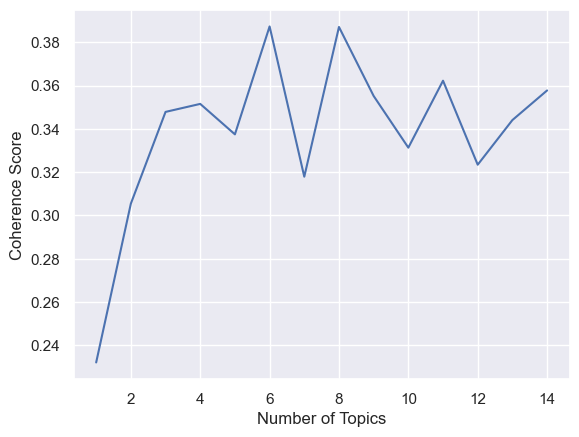
\includegraphics[width=\textwidth]{cv.png}
    \caption{Coherence for $c_v$ approach}
    \label{cv}
\end{subfigure}
\hfill
\begin{subfigure}{0.45\textwidth}
    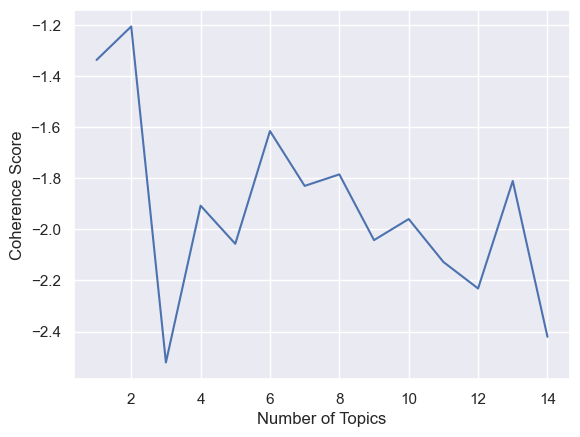
\includegraphics[width=\textwidth]{umass.png}
    \caption{Coherence for $u_{mass}$ approach}
    \label{umass}
\end{subfigure}       
\caption{Coherence score to estimate optimal number of Topics}
\label{cv_umass}
\end{figure}

From the chart we can see that six topics are dominant in our provided
corpus. The chart shown at the left shows the coherence score for
\(u_{mass}\) and the right chart represents the score for \(c_{v}\) for
multiple iterations. Using 6 topics we can see the output of
corresponding topic and top 10 words in a topic.



\textbf{Topic 01}: {[}\enquote*{energy} 0.060, \enquote*{source} 0.029, \enquote*{renewable} 0.018, \enquote*{water}
0.016, \enquote*{use} 0.013, \enquote*{gas} 0.013, \enquote*{produce} 0.013, \enquote*{green} 0.013, \enquote*{warm}
0.013, \enquote*{cause} 0.012,{]}

\textbf{Topic 02}: {[}\enquote*{pastime} 0.024, \enquote*{computer} 0.024, \enquote*{social} 0.023, \enquote*{user}
0.022, \enquote*{network} 0.020, \enquote*{student} 0.019, \enquote*{class} 0.017, \enquote*{change} 0.016,
\enquote*{book} 0.015, \enquote*{survey} 0.013,{]}

\textbf{Topic 03}: {[}\enquote*{mother} 0.083, \enquote*{buy} 0.021, \enquote*{love} 0.018, \enquote*{child} 0.014,
\enquote*{worker} 0.014, \enquote*{begin} 0.013, \enquote*{cultural} 0.012, \enquote*{observe} 0.012,
\enquote*{thing} 0.012, \enquote*{language} 0.011,{]}

\textbf{Topic 04}: {[}\enquote*{life} 0.016, \enquote*{Bangladesh} 0.016, \enquote*{family} 0.015, \enquote*{home}
0.014, \enquote*{root} 0.014, \enquote*{language} 0.014, \enquote*{country} 0.013, \enquote*{Pakistan}
0.010, \enquote*{war} 0.010, \enquote*{man} 0.009,{]}

\textbf{Topic 05}: {[}\enquote*{country} 0.031, \enquote*{river} 0.022, \enquote*{India} 0.022, \enquote*{land} 0.021,
\enquote*{boat} 0.015, \enquote*{small} 0.015, \enquote*{population} 0.015, \enquote*{lake} 0.013, \enquote*{group}
0.012, \enquote*{house} 0.011,{]}

\textbf{Topic 06}: {[}\enquote*{job} 0.064, \enquote*{English} 0.023, \enquote*{learn} 0.021, \enquote*{teacher}
0.017, \enquote*{use} 0.016, \enquote*{dream} 0.016, \enquote*{think} 0.016, \enquote*{thing} 0.015,
\enquote*{school} 0.014, \enquote*{education} 0.013{]}

\subsection{Count vs Relative Importance measurement}

Word frequency $n(w_{j},d_{i})$ in each document \(D\) is measured as below which identifies the most frequent words within each document and across the entire corpus.

\(D = \sum_{d_{i} \in D}^{}\left\{ \begin{matrix}
1,n\left( w_{i},d_{i} \right) > 0 \\
0,n\left( w_{i},d_{i} \right) = 0 \\
\end{matrix} \right.\ \)

we can visualize relative importance of any keywords in terms of frequency and plotted inclined with LDA provided weights.

\begin{figure}[h]
\centerline{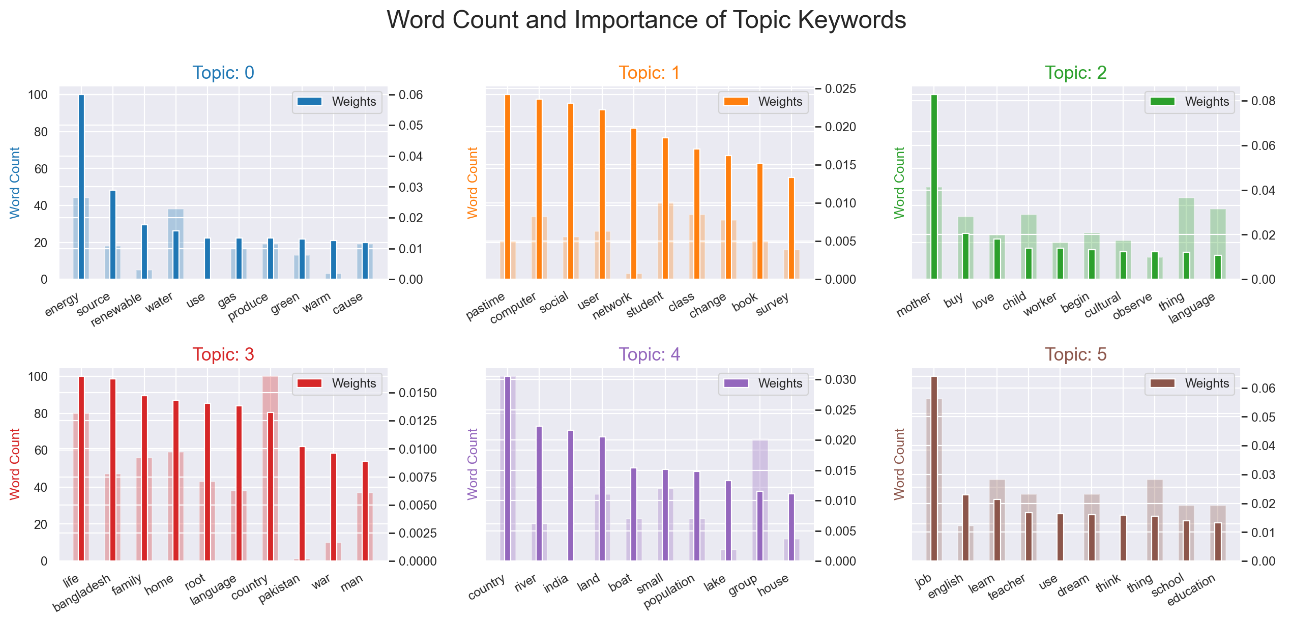
\includegraphics[width=\textwidth]{relative_imp.png}}
\caption{Word frequency and its relative importance}
\label{fig:Relative_weight}
\end{figure}

\section{Dominant topic and contribution}

In LDA models, each document is composed of multiple topics. But
typically, some specific topics are dominant. The following experiment
extracts this dominant topic for each sentence and shows the relative
weight of the topic and the keywords. It estimated which document
belongs predominantly to which topic. How frequently the words have
appeared in the documents and the weights of each keyword in the same
chart, words that occur in multiple topics and the ones whose relative
frequency is more than the weight.

\subsection{Topic-Term Matrix Visualization and Inter-Topic Distance Map}

Visualizing the topics and their relationships in a topic model Python
library PyLDAvis is used provides an interactive web-based interface to
explore and analyze the LDA results of topic modeling. PyLDAvis itself
abstracts away much of the underlying mathematical complexity and
provides a user-friendly way to generate visualizations and
interactively explore topics and their relationships. Key components
distance among topics and salient terms are explained below:

\subsubsection{Inter-Topic Distance Map}

Distance among topics refers to the measurement of similarity between
topics in a high dimensional space matrix provided by the LDA model.
PyLDAvis library is used to conserve dimensionality reduction using PCA
and for calculating distance between topics metric like Euclidean
distance or Cosine Similarity \(\). Topic-topic distribution matrix
\(Q\left( t_{1},t_{2} \right)\) for topic \(t_{1}\) and topic \(t_{2}\),
distance \(D\)between \(t_{1},t_{2}\) can be represented as

\subsubsection{Salient Terms or dominant keywords}

Salient Terms in a topic are words \(W\) that are most strongly
associated with specific topic. The mathematical expression for finding
salient terms \(w\) for a topic \(t\) involves, extraction of top
\(n\)words that poses the highest probability scores for topic \(t\) in
the topic-term matrix \(P\lbrack t,w\rbrack\).

\begin{figure}[h]
\centerline{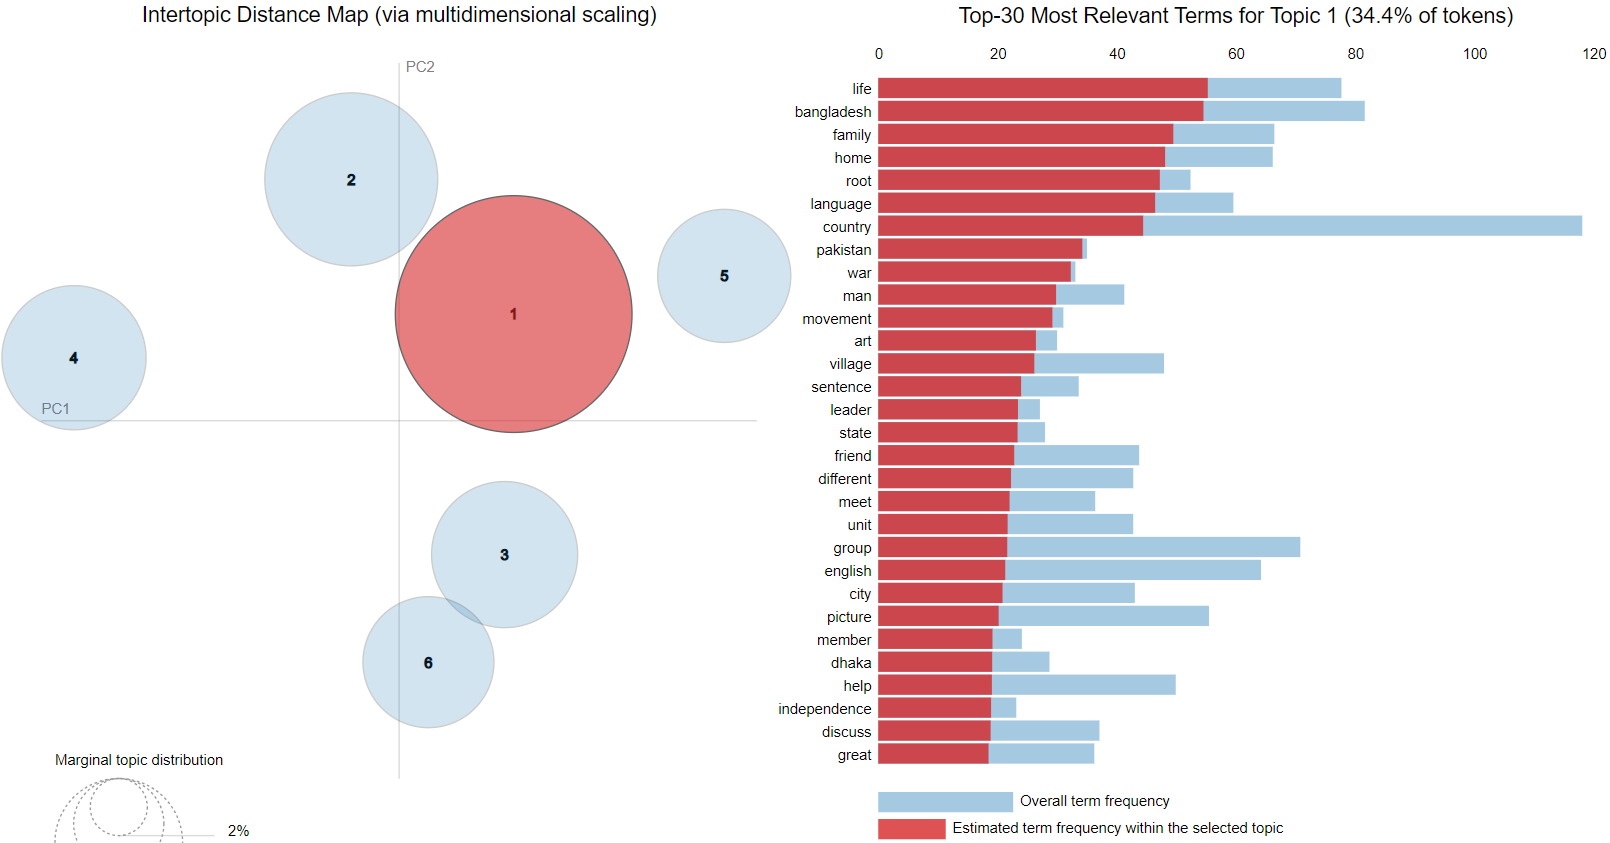
\includegraphics[width=\textwidth]{pyldvis.png}}
\caption{Topic model co-occurrence visualization with dominant keywords'}
\label{fig:Relative_weight}
\end{figure}

Top 30 most salient terms are showed at right in the bar chart histogram
and left figure shows inter topic distance, their size etc. PCA
dimensionality reduction technique is applied here to embed the LDA
result into a 2D plain scale. Projected the data in lower-dimensional
subspace by computing eigenvalues reduced the circle overlapping. Topics
that are closer together in the map are more similar in terms of the
distribution of words.

\section{Englisher Mobile App}
A mobile application (Englisher) is being developed with content from the NCTB’s English Textbook for class 9. The extracted keywords are organized into lessons and furthermore quiz is introduced as an exercise. Each sentence's and word's Bengali meaning is provided in accordance with the lesson. Students can take quizzes, and their results are recorded in the history so that history can be reviewed and performance can be improved by more practice in the future. 

\begin{figure}[h!]
\centering
\begin{subfigure}{\textwidth}
	\centering
    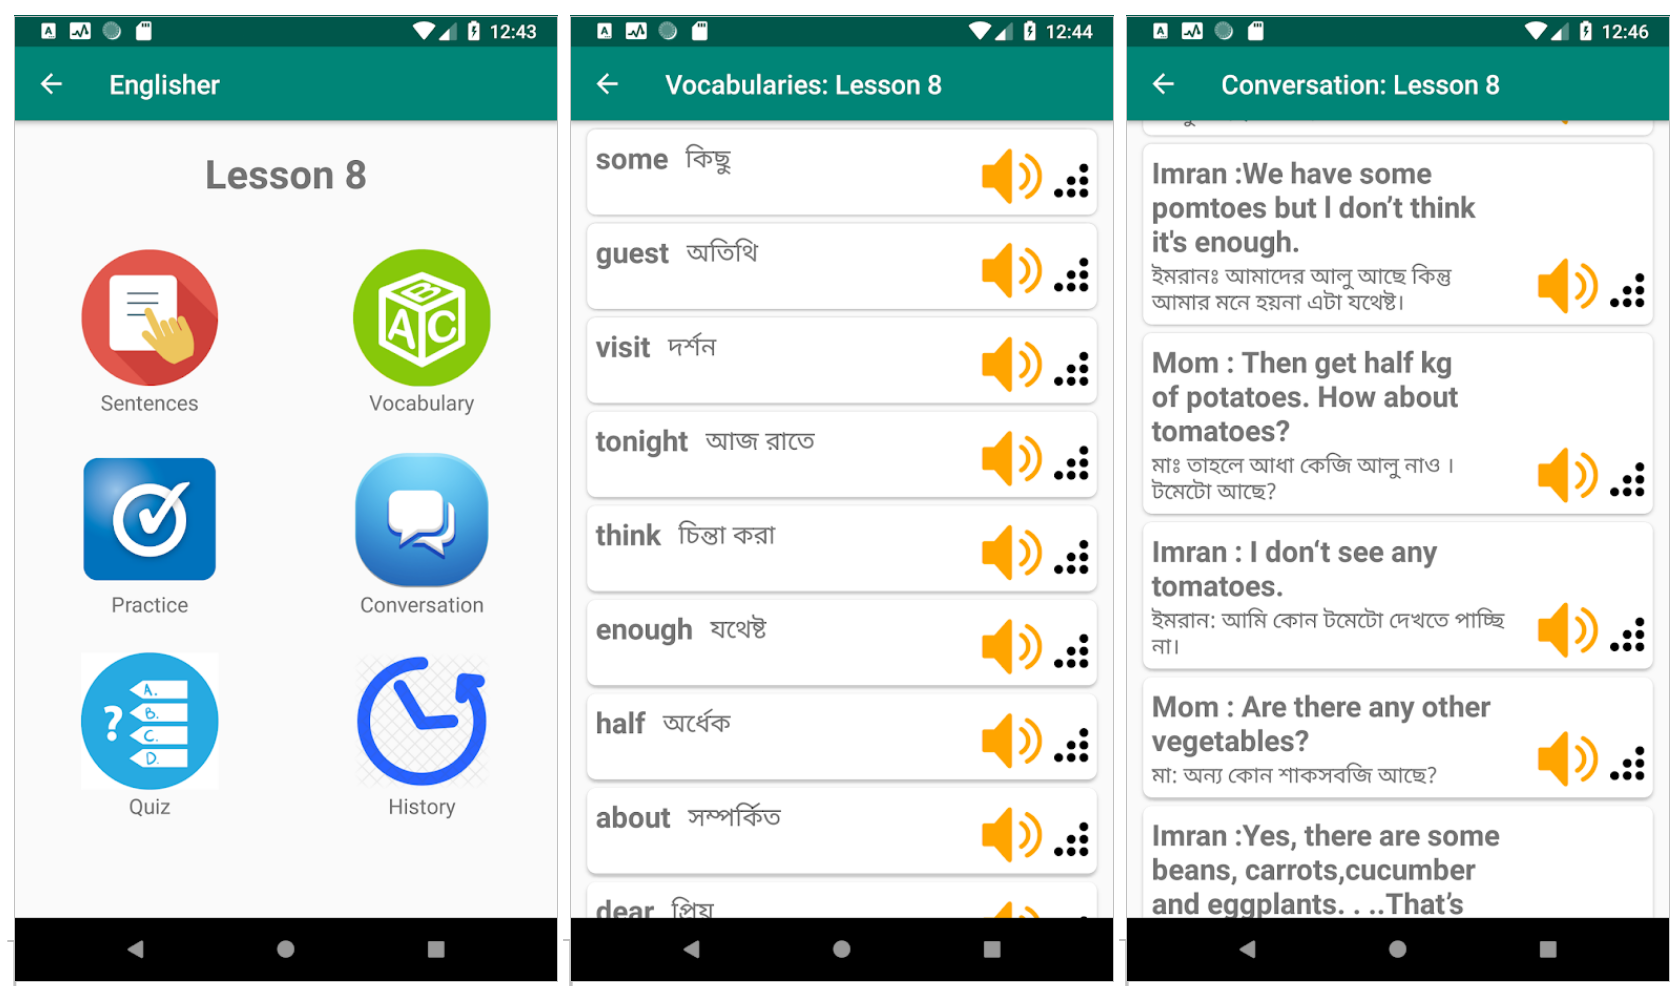
\includegraphics[width=\textwidth]{mobile_app_01.png}
    \caption{Lesson wise exercise}
    \label{fig:first}
\end{subfigure}
\hfill
\begin{subfigure}{\textwidth}
	\centering
    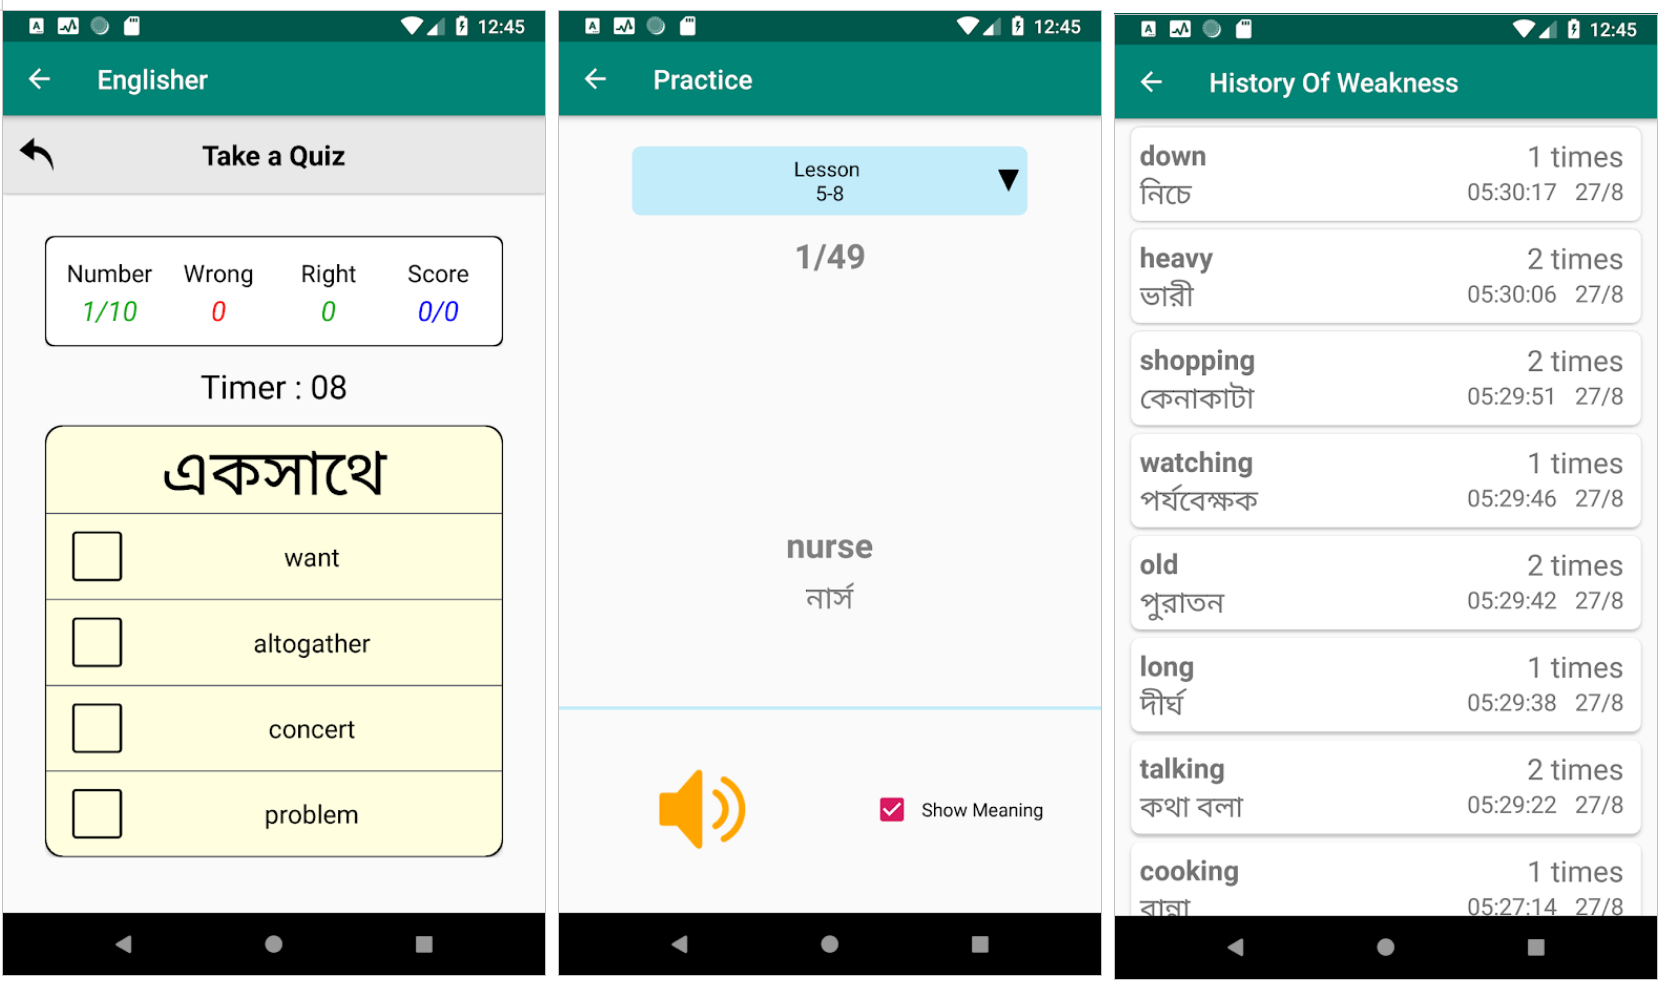
\includegraphics[width=\textwidth]{mobile_app_02.png}
    \caption{Quiz with Vocabulary}
    \label{fig:second}
\end{subfigure}
        
\caption{Englisher Mobile app for Learning LDA based topic model words}
\label{fig:figures}
\end{figure}

\section{Qualitative survey}
In the survey questions, it was indicated whether the students, teachers/instructors, and government organizations would find it acceptable and appreciated if textbook information were made available through a mobile app and presented in interactive format. To demonstrate the mobile app idea during the interrogation survey session prototype app Englisher is prepared. Participants were asked for suggestions on how to make the app better and specify shortcomings. Presumably It provides an insight of teacher’s emotion about inclusion of mobile technology in higher secondary English education system. 

\subsection{Survey Planning}
The survey was conducted over a period of four weeks, with 50 High schools in Dhaka and Bogura district of Bangladesh. It encompasses only English subject areas Teachers who teaches in high schools from class six to class Ten and teaches regularly in the school. A questionnaire was distributed to teachers allowing us to gather questionnaire answer. 
\subsubsection{Survey participants}
During the survey standard participants were chosen emphasizing infrastructure quality, teaching experience, class size etc. At the beginning from 100 institution were selected. Then half of them were excluded since those institutions infrastructure's overall quality and condition were not above average. Among the chosen samples 76\% were good and 26\% considered average institutions. Privately held 45\%, 32\% partially government and 22\% are government institutes.  Over 1000 students study in almost 40\% of these institutions and  sizable number of pupils are present in each section and class. 38\% class have a size greater than 50. So, we can presume that the participating teachers have quite a bit of experience teaching sufficient number of students.  
\subsection{Survey Results:}
We have done extensive analysis with the survey data collected. In our data collection highest priority is given for the secondary class student teachers who teach between 6-10th class about 46\%. High school, KG college and KG High school. Details about the statistics are depicted in the following figure. Adjacent chart explains the percentage of teachers who teach in which class. Hence, from these two figures we can get a vivid image of collected dataset resources about the participating teachers. 


\subsection{Training Dataset}
In this research we have used dataset from \cite{gaur2019knowledge}. For training classifier in this research 2019's Gaur et. al \cite{gaur2019knowledge} dataset is used. Compared to the existing four-label classification scheme (no risk, low risk, moderate risk, and high risk), this dataset introduced 5 lavel classification suicide indicator, ideation, behavior, attempt and another extra category incorporating supportive category. Supportive category represents whenever someone shows empathy and condolance for a suicidal post. 

\subsection{Testing/Validation Dataset} 
For testing dataset is collected from kaggle. It is an opesource dataset publicly available collected from reddit website by a pushshift API contained suicide and depression category.  This publicly available Reddit datasets in Kaggle Website comprised of 232,074 post annotated for binary classification as suicidal or non-suicidal in \cite{aldhyani2022detecting} for detecting suicidal ideation. The dataset is a collection of posts from the "SuicideWatch" and "depression" subreddits of the Reddit platform. All posts that were made to "SuicideWatch" from Dec 16, 2008(creation) till Jan 2, 2021, were collected while "depression" posts were collected from Jan 1, 2009, to Jan 2, 2021. In this research trained classifier is applied to detect class on this two category. Main objective isto determine the suicide categories (indicator, ideation, behavior, attempt, supportive ) within this dataset. Document length frequency and token distribution is depicted in Figure \ref{redditdist}. From the frequency distribution we can see some of the document sizes are very large. Hence, during the training process we chopped the sentences into multiple sentences keeping the label same. 

\subsection{Data Processing and Models}
\subsubsection{Data Pre-processing}\label{data_preprocessing}
Social media dataset are mostly Text data which needs data pre-processing, cleaning, feature extraction and data mining related NLP tasks. NLP based text data contains noises such as: unnecessary quotes, special characters, punctuation etc. Moreover, morphological analysis is needed to retrieve root words followed by stemming, lemmatization. Then, sentences are divided into equal-length fragments, and null word padding is applied as needed. Words within a phrase are now referred to as tokens or features, and the dataset is shown as a corpus. Special features/tokens are further preprocessed and filtered using text data feature extraction tools and methods. Features are passed through a process in which features are converted to corresponding IDs and sentences which contains a series of IDs are represented a vector. The embedding is another term that is frequently used in relation to vector text analysis. Various Vectorization methods are present. Traditional vectorization method provide weights to terms/words mainly based on frequency of words within the sentence and documents, rather than its importance and contextual meaning. Also, how does a particular word or term create impact on the neighboring words is not taken into consideration, since these models does not have any prior knowledge of any words. Hence, various neural network based language models are proposed which are pretrained on massive amount of dataset. These models mainly carries weight which represents word to word relationships and most cases can provide contextual meaning of given sentence based on pretrained dataset knowledge. Deep learning models recently showed remarkable achievements in this case representing corresponding knowledge.

\subsubsection{Classification}
Machine learning and Deep Learning models are particularly used for Text classification and ML for feature selection or extraction in several studies \cite{castillo2020suicide, chancellor2020methods, zhang2022natural}. These extensive reviews reveal Deep learning methods receive more attention and perform better than traditional machine learning methods whereas in some cases when extracted or filtered features are fit into training process models are able to perform better. NLP techniques are applied for the annotated dataset collected from Twitter, Reddit, Facebook, instagram, Weibo \cite{wang2020depression} etc. After that various deep learning and machine learning models are trained for classification of suicide and depression. Then trained models are applied to determine the correct class of given text. \cite{malhotra2022deep} Provided a through investigation about passed research techniques, features, datasets, and performance metrics \cite{zhang2022natural, chancellor2020methods}. 

\subsubsection{Data Learning Models}
Among Several Deep Learning approaches most successful NLP classifier for segregating Depression and suicidal task are CNN, LSTM, GRU, XLNET, BERT, Variants of BERT RoBERTa and variants of CNN such as: CNN-BiLSTM etc \cite{aldhyani2022detecting, wang2020depression, shetty2020predicting} also showed promising results. 

\subsubsection{Feature Selection} 
The feature selection procedure has a substantial impact on the performance of machine learning and deep learning models because it lowers noise in the trained dataset, enabling the model to accurately understand data patterns. LIWC, LDA, LSA, n-gram analysis \cite{pennebaker2001linguistic, tadesse2019detection} etc are used as features analysis tools. 
Most dominant approaches are n-gram word frequency based approach TF-IDF. Apart from the Deep learning model n-gram Traditional feature retrieve based analysis conducted in some research papers. In 2017 Shen et. al \cite{harvesting_social_media} collected several forms of features comprised of six chorots, namely, social network features, user profile features, visual features, emotional features, topic-level features, and domain-specific features and prepared a feature rich dictionary. This multimodal depressive dictionary learning model was used to detect the depressed users on Twitter using machine learning models. 

Most dominant approaches are Word2Vec, XGBoost, SVM, Random Forest, other regression MLs. Typical word embedding approaches TF-IDF and Word2Vec, and CNN–BiLSTM are applied in  \cite{aldhyani2022detecting}. Using LIWC features, XGBoost ML together surpasses the accuracy of CNN–BiLSTM in  \cite{aldhyani2022detecting}. Others have used machine text Summarization based feature extraction strategy followed by classification for depression detection is applied in \cite{zogan2021depressionnet}. \cite{burnap2015machine}built a set of baseline classifiers using lexical, structural, emotive and psychological features extracted from Twitter posts. Then baseline classifiers are updated by building an ensemble classifier using the Rotation Forest algorithm and a Maximum Probability voting classification decision method. \cite{chancellor2020methods} This paper provided an excellent overview of 75 studies in between 2013 and 2018 outlining the methods of data annotation for mental health status, data collection and quality management, pre-processing and feature selection, and model selection and verification. 

\subsection{Other Tools or Methods}
Apart from the Machine Learning or statistical model approaches there are some sites, helpline numbers and apps \cite{martinengo2019suicide} that contains various facts, statistics, tips, tools, healthline numbers and ways to handle suicidal depression \cite{suicidaldepression_online}. 
  
nce, visualizing the result we can determine the suicidal tendency within depression post. Also, N-gram based analysis is conducted and frequency of Terms and connections of words or phrases are analyzed in this research scope. More often topic modeling clustering is used to determine latent topic and understand latent text network. From the network various facts can be revealed related to suicide and depression. This whole process is depicted in Figure \ref{fig:res_diagram}


\section{Results Analysis}\label{sec2}
First we started our experiment with document length distribution. The length of document and term frequency within the corpus is visualized in Figure \ref{redditdist_twitterdist}. From the distribution we can see that some of the document length are excessive long and contains more than 1000 tokens ( within Twitter and also Reddit both Dataset). Depression class document length are usually shorter in length. Depression document length are tend to be smaller than suicide document length. 

Short sentence does not carry much terms and hence does not carry enough information to be classified confidently by classifier algorithms. We started reducing the numbers of samples based on document length. By reducing the samples based on numbers of tokens present in a document (see Figure \ref{redditdist_twitterdist}). Documents length versus category frequency information is showed in this chart. This charts explains if we filter out the shorter comments suicide post become dominant class and depression post become outnumbered. The difference showed an exponential pattern as length of document increases. Test dataset Reddit data distribution among depression and suicide class distribution ratio is equal. Filtering the class we have seen an interesting fact that depressed people does not want to comment very long. 



\subsection{N-gram Analysis}
\subsubsection{Uni-gram}
Dataset is split into separate tokens after preprocessing and uni-gram generated. Based on frequency of words wordcloud is generated from these unigrams. Frequency based comparison between two categories is conducted for depression and suicide for Test dataset in Figure \ref{features_vis_pro_exp}. Main objective was to get top ranked words from Depression and Suicide corpus. After experiments we have seen There are similarities between the top ranked words those are occurring frequently. They tend to use slang and abusive terms compared to suicidal attempt thinking people. Rather suicidal depressed people want to share their thoughts with others using longer post. However, it does not reveals any clues in terms of hypothetical relationships between the two category. It is difficult find pattern in which we can determine the depression and suicidal thought. So far we found some pattern 
%\begin{enumerate}
%\item short statements likely to be more depression category
%\item Depressive statements tend to have slang
%\item Suicidal thinking people’s post having very high frequency of “kill” “die” these type of words or phrases.
%\end{enumerate}
%
%\begin{figure}[H]
%\centering
%\begin{subfigure}{0.45\textwidth}
%    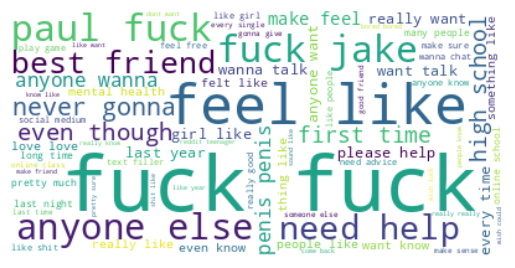
\includegraphics[width=\textwidth]{dep_wordcloud.png}
%    \caption{Wordcloud in Depression category}
%    \label{fig:first}
%\end{subfigure}
%\hfill
%\begin{subfigure}{0.45\textwidth}
%    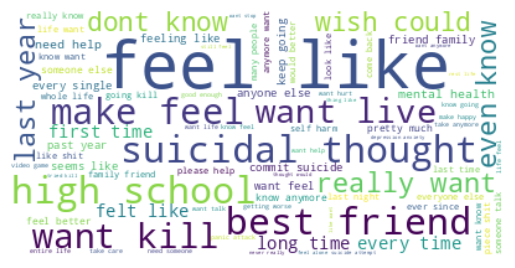
\includegraphics[width=\textwidth]{sui_wordcloud.png}
%    \caption{Wordcloud in Suicide category}
%    \label{fig:second}
%\end{subfigure}
%\hfill
%\begin{subfigure}{0.8\textwidth}
%    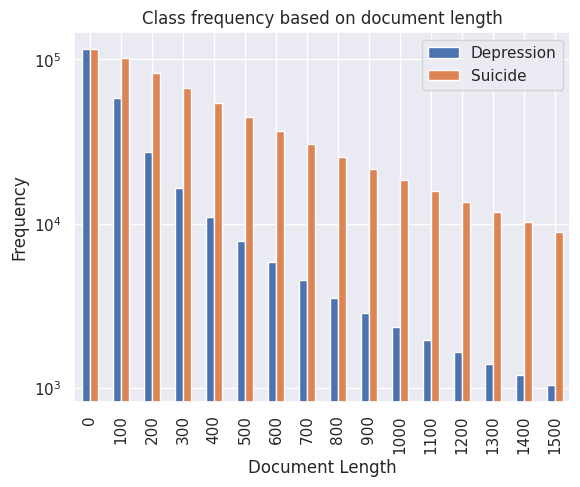
\includegraphics[height=7.5cm, width=\textwidth]{doc_len.png}
%    \caption{Class frequency in different Document Length}
%    \label{fig:second}
%\end{subfigure}        
%\caption{Dataset features visualization and properties exploration}
%\label{features_vis_pro_exp}
%\end{figure}

To understand the term occurring frequently in two different classes scatterplot library is used for visual analysis. From the above two scenario we can see that there is a pattern that people used to say more slang and abusive words when they are depressed. It is also interesting that there are many words have high frequency such as depression or depressed but belongs to suicide class. One important fact is revealed here is that we can see although suicide, suicidal these words has high frequency in Suicide class but depression, depressed also occurred in parallel with high frequency. Here several experiments can be conducted for exploratory analysis with scattertext library for terms significance. However, this library is computationally heavy for larger dataset for visualization. Another drawbacks is this library have significant focus on the terms based analysis. We have used simple vectorization methods by which we can have greater control on dataset and experiments code. 

\subsubsection{Bi-gram}
First unigram is computed and analyzed then bigram is calculated for both categories. The bigram frequency showed there are some common terms like “mental health”, “feel like”, “make feel”, “high school” etc showed high occurrences in the dataset. Hence, we started to understand its pattern in the corpus. For analysis we have considered ['high school', 'mental health', 'best friend', 'feel like', 'really want', 'suicide thought', 'friend family'] these bi-grams and wanted to explore its surrounding context for each category. We called this special bigrams since it showed importance in the suicidal and depression both categories appeared highly frequent matter. We want to analyze how these words have impact with its neighboring words. 

To explore the impact of special bi-grams on the samples, special bi-gram terms containing samples are filtered from dataset. After that using lebel encoder bigrams are encoded as integers and then chord diagram is generated  depicted in Figure \ref{Bigram_features_exp} to find meaningful relationship within the samples between the bigram features.  


%\begin{figure}[H]
%\centering
%\begin{subfigure}{0.8\textwidth}
%    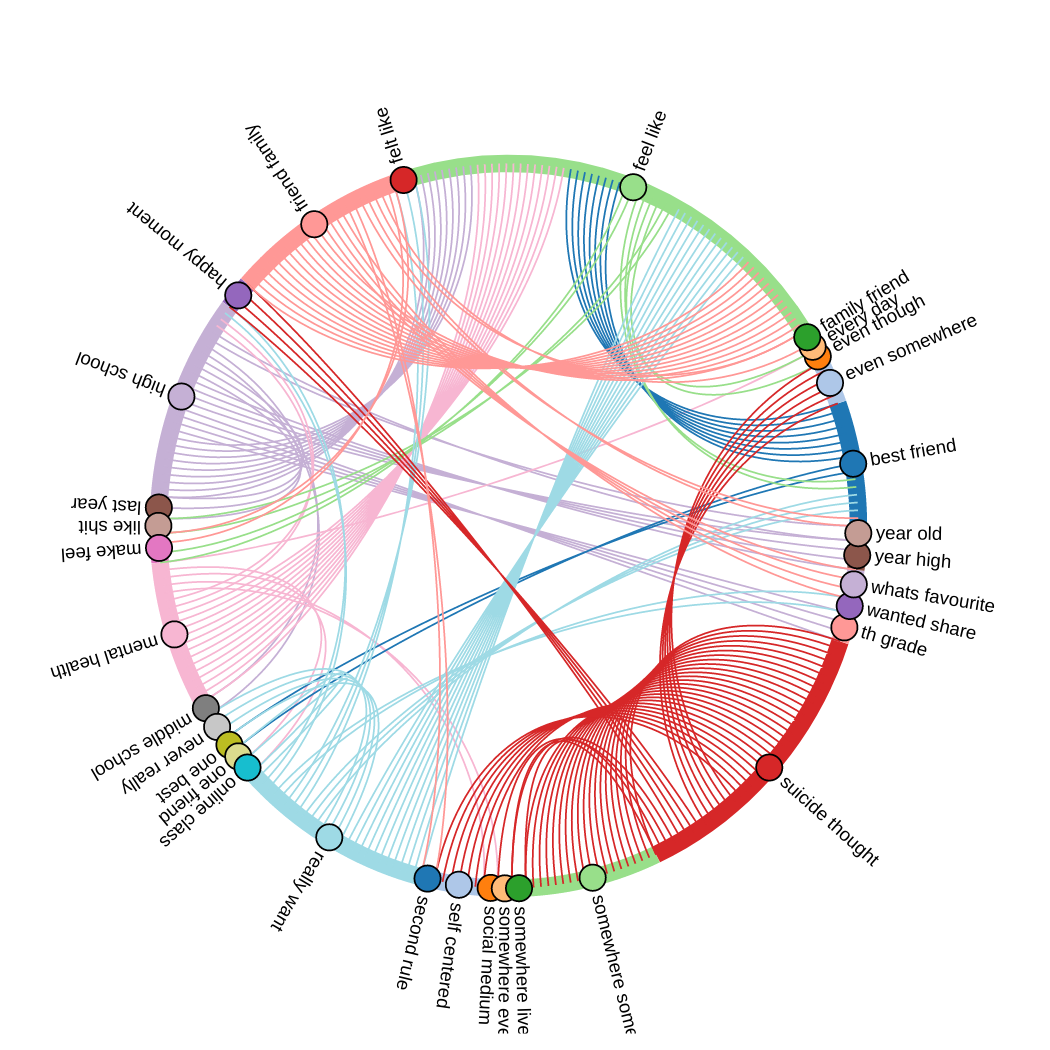
\includegraphics[width=\textwidth]{dep_chord.png}
%    \caption{Depression Chord diagram}
%    \label{fig:first}
%\end{subfigure}
%\hfill
%\begin{subfigure}{0.8\textwidth}
%    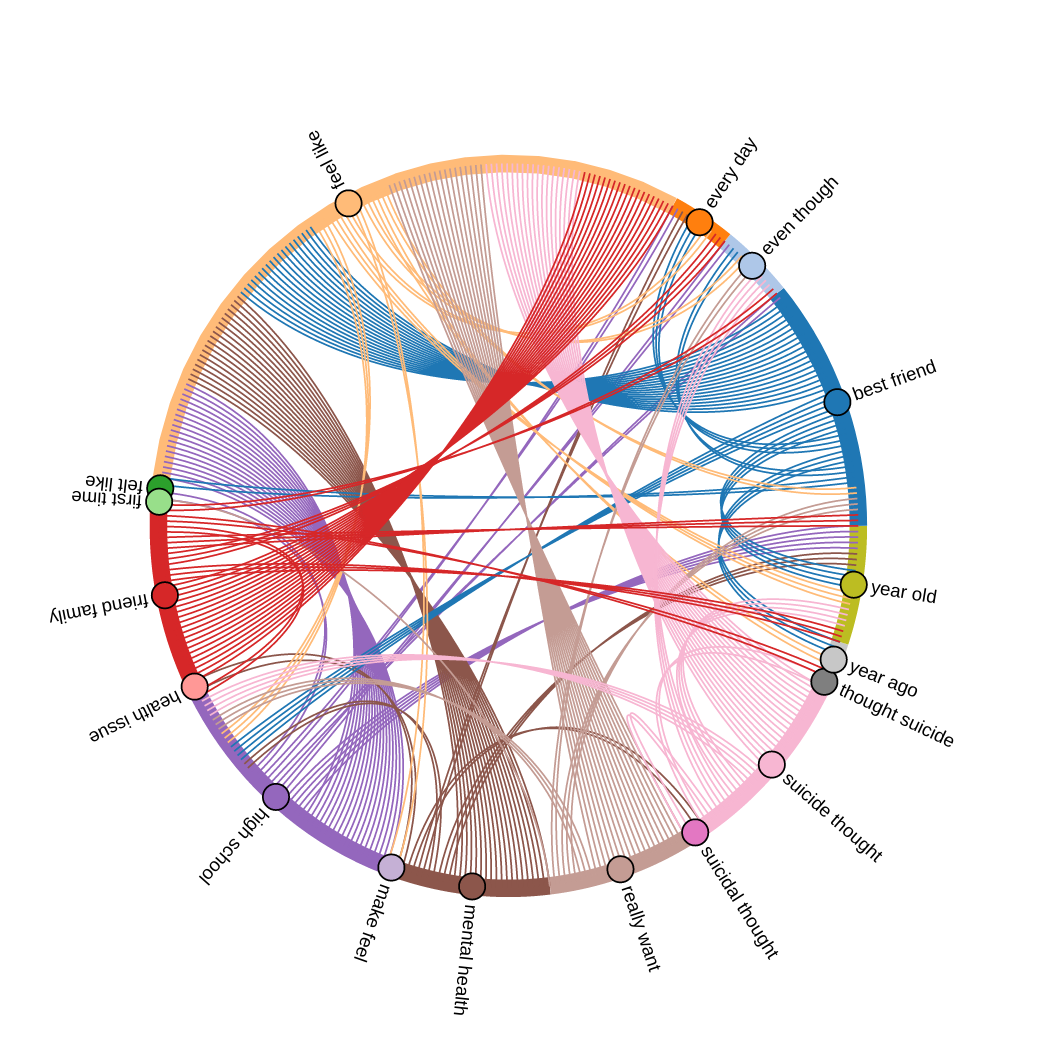
\includegraphics[width=\textwidth]{suicide_chord.png}
%    \caption{Depression Chord diagram}
%    \label{fig:second}
%\end{subfigure}        
%\caption{Bi-gram features relation exploration}
%\label{Bigram_features_exp}
%\end{figure}


From this two chord diagram interesting sentence can be inferred. Such as: from the depression class ? self centered person is depressed, having suicidal thought, want to go somewhere to live, spend happy moments and so on. For the suicidal class category suicidal attempt thinking people, have mental health issue, they want to share though with high school friends, best friends, friends and family members, having suicidal thoughts and so on.  

Tri-grams or above did not reveals much meaning information, mostly does convey some meaningful information and therefore excluded for further experimental consideration. 

\section{Classification Results}
To segregate the Reddit suicide dataset into different categories of suicide first we have created a classifier using different classification techniques. Since our objective is not making highly accurate classifier. Following approach is applied in this study

\begin{itemize}
\item Pre-processed and useful features are used from Twitter's 500 post CSSR dataset for Training classifier
\item Used count vectorizer and TFIDF transformer to generate vectors for the dataset
\item Trained classifier to determine the categories of various suicidal intensities
\end{itemize}

We have used simple gridsearch technique of sklearn library and from a list of various classifiers applied on the dataset, we have chosen highest accurate classifiers to determine different label of suicidal risk. so that it can recognize the category. We have used classifiers "K Nearest Neighbors", "Linear and RBF SVM", "Gaussian Process", "Decision Tree", "Random Forest", "Vanilla Neural Net", "AdaBoost", "Naive Bayes". Using various set of parameters, from the result and experiments we found almost 60\% accuracy for SVM model to predict the suicide intensity categories. From various set of values of SVM we found degree=2, gamma=0.7, kernel=rbf showed the highest accuracy. 


%\begin{table}[h]
%\begin{center}
%\begin{minipage}{174pt}
%\caption{Caption text}\label{tab1}%
%\begin{tabular}{@{}lllll@{}}
%\toprule
%Classifier & Precision & Recall & Accuracy & F1 \\
%\midrule
%Nearest Neighbors & 0.926 & 0.924 & 92.3896 & 0.924\\
%RBF SVM & 0.942 & 0.924 & 92.3896 & 0.927\\
%Decision Tree & 0.901 & 0.848 & 84.7793 & 0.856\\
%Random Forest & 0.513 & 0.282 & 28.1583 & 0.167\\
%Neural Net & 0.942 & 0.927 & 92.6941 & 0.929\\
%AdaBoost & 0.905 & 0.898 & 89.8021 & 0.899\\
%Gaussian Process & 0.940 & 0.921 & 92.0852 & 0.924\\
%Naive Bayes & 0.923 & 0.918 & 91.7808 & 0.919\\
%QDA & 0.931 & 0.909 & 90.8676 & 0.912\\
%\botrule
%\end{tabular}
%\footnotetext{Shows classifiers accuracy of classification models}
%\end{minipage}
%\end{center}
%\end{table}

\subsubsection{Suicidal Intensities visualization}
How much depression can trigger suicidal thoughts is an interesting question. In this study classifier is trained on the suicidal intensity. Then trained classifier is applied on the Depression/Suicide class dataset. From various machine learning models we have found SVM is a good performing model. SVM classifier is applied for the TFIDF vectorizer embedding (see results in figure~\ref{SVMTFIDF}) and also for Word2vec pretrained vectorizer model. The results are shown in figure~\ref{Suicidal_int_vis}. From the results we can see that suicidal ideation between depression and suicidal categories number of samples are very similar. Within depression more number of samples are showed suicidal indicator category compared to suicide which is an interesting result. Suicidal behavior and attempt is comparatively high within the suicidal category than depression. Hence, figure~\ref{SVMTFIDF} result seems to be pretty obvious, except for suicidal ideation category. Also for the suicidal indicator symptoms are higher within the depression category. 

%\begin{figure}[H]
%\centering
%\begin{subfigure}{0.45\textwidth}
%    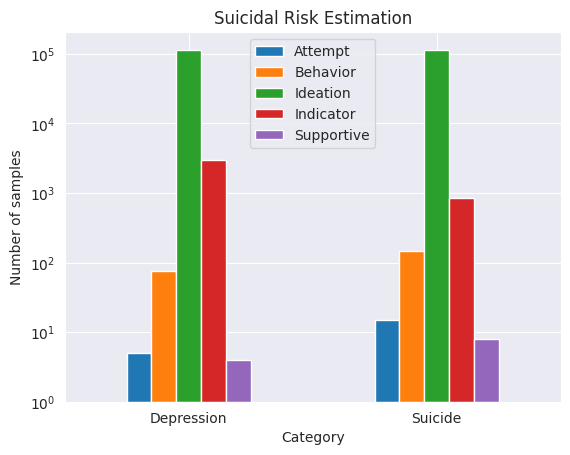
\includegraphics[width=\textwidth]{grid_svm.png}
%    \caption{SVM classifier applied for TFIDF vectorizer}
%    \label{SVMTFIDF}
%\end{subfigure}
%\hfill
%\begin{subfigure}{0.45\textwidth}
%    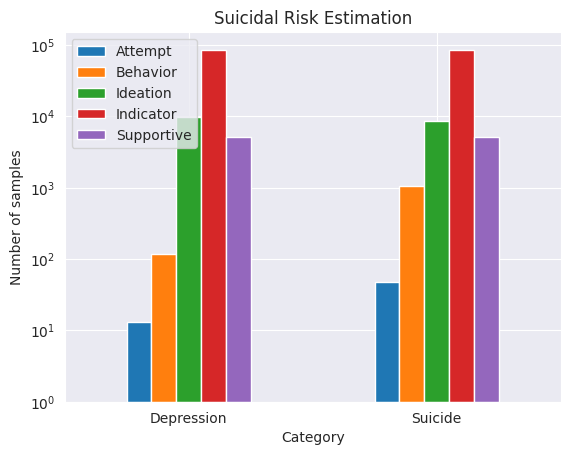
\includegraphics[width=\textwidth]{glove_vec.png}
%    \caption{SVM classifier applied for Glove Word2Vec Pretrained model vectorizer}
%    \label{GloveWord2Vec}
%\end{subfigure}        
%\caption{Visualizing suicide intensities within Depression/Suicide class}
%\label{Suicidal_int_vis} 
%\end{figure}

For the word2vec vector embedding scenario supportive and indicator categories results are almost similar in depression or suicide both classes. There is slight difference is shown for suicidal ideation and within suicide class, suicidal ideation is slight higher. Except the behavior and attempt category for the rest categories depression and suicide showed almost similar number of samples. 

%\begin{figure}[H]
%\centering
%\begin{subfigure}{0.45\textwidth}
%    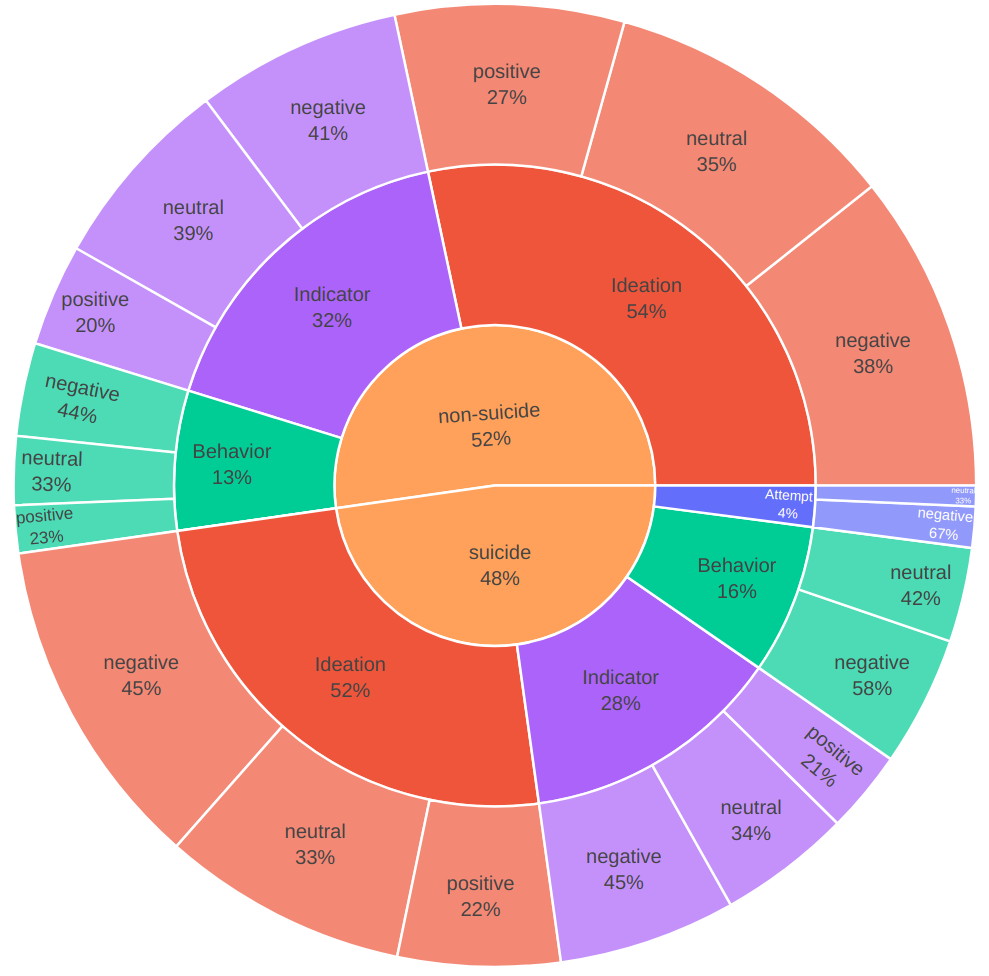
\includegraphics[width=\textwidth]{sentiment_sunburst.png}
%    \caption{First subfigure.}
%    \label{fig:first}
%\end{subfigure}
%\hfill
%\begin{subfigure}{0.45\textwidth}
%    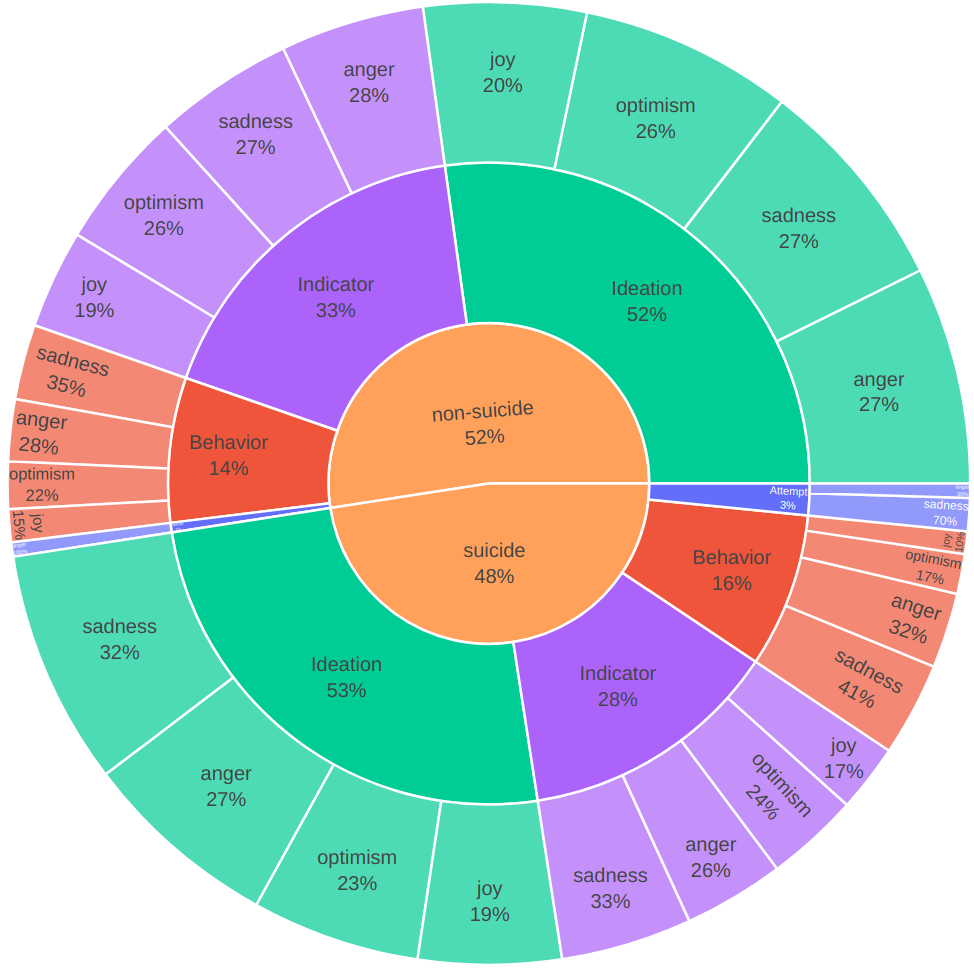
\includegraphics[width=\textwidth]{emotion_sunburst.png}
%    \caption{Second subfigure.}
%    \label{fig:second}
%\end{subfigure}
%        
%\caption{Subreferences in \LaTeX.}
%\label{fig:figures}
%\end{figure}
\section{Discussion} 
From the result it is revealed that suicide categories shown within depression and suicide class vividly. Specially suicidal ideation, indicator showed similar patterns. The number of samples within depression and suicide is almost similar for this two categories. Hence, we can infer depressed person comments showed suicidal ideation and suicidal indicating symptoms. Suicidal behavior and attempt showed higher number of samples within the suicide category compared to depression category. All these results seems very logical results. Although from the results mathematical formulas are not derived in this research study since results are susceptible to chosen classifier, chosen dataset, pretrained models vectors or embedding provided to the classifier. 
 
\section{Conclusion}
Suicidal risk estimation task and classification samples to determine suicidal risk within social websites and blogs, techniques are discussed before. According to suicidal category previous work has been done before. However, to what extent depression level triggers suicidal risk is not yet discussed before. Also it is difficult to determine since depression and suicide categorical variables are independent factor. There is not any underlying correlation. Several research conducted to segregate which post is suicidal and which one is depression various classifiers are proposed. Extensive work has been done to improve the classification accuracy by adopting most powerful vectorization techniques that uses cutting edge NLP models BERT and its various variants. Research has also been conducted on how much severity label of suicide within a post is studied. 

%\section{This is an example for first level head---section head}\label{sec3}
%
%\subsection{This is an example for second level head---subsection head}\label{subsec2}
%
%\subsubsection{This is an example for third level head---subsubsection head}\label{subsubsec2}
%
%Sample body text. Sample body text. Sample body text. Sample body text. Sample body text. Sample body text. Sample body text. Sample body text. 
%
%\section{Equations}\label{sec4}
%
%Equations in \LaTeX\ can either be inline or on-a-line by itself (``display equations''). For
%inline equations use the \verb+$...$+ commands. E.g.: The equation
%$H\psi = E \psi$ is written via the command \verb+$H \psi = E \psi$+.
%
%For display equations (with auto generated equation numbers)
%one can use the equation or align environments:
%\begin{equation}
%\|\tilde{X}(k)\|^2 \leq\frac{\sum\limits_{i=1}^{p}\left\|\tilde{Y}_i(k)\right\|^2+\sum\limits_{j=1}^{q}\left\|\tilde{Z}_j(k)\right\|^2 }{p+q}.\label{eq1}
%\end{equation}
%where,
%\begin{align}
%D_\mu &=  \partial_\mu - ig \frac{\lambda^a}{2} A^a_\mu \nonumber \\
%F^a_{\mu\nu} &= \partial_\mu A^a_\nu - \partial_\nu A^a_\mu + g f^{abc} A^b_\mu A^a_\nu \label{eq2}
%\end{align}
%Notice the use of \verb+\nonumber+ in the align environment at the end
%of each line, except the last, so as not to produce equation numbers on
%lines where no equation numbers are required. The \verb+\label{}+ command
%should only be used at the last line of an align environment where
%\verb+\nonumber+ is not used.
%\begin{equation}
%Y_\infty = \left( \frac{m}{\textrm{GeV}} \right)^{-3}
%    \left[ 1 + \frac{3 \ln(m/\textrm{GeV})}{15}
%    + \frac{\ln(c_2/5)}{15} \right]
%\end{equation}
%The class file also supports the use of \verb+\mathbb{}+, \verb+\mathscr{}+ and
%\verb+\mathcal{}+ commands. As such \verb+\mathbb{R}+, \verb+\mathscr{R}+
%and \verb+\mathcal{R}+ produces $\mathbb{R}$, $\mathscr{R}$ and $\mathcal{R}$
%respectively (refer Subsubsection~\ref{subsubsec2}).
%
%\section{Tables}\label{sec5}
%
%Tables can be inserted via the normal table and tabular environment. To put
%footnotes inside tables you should use \verb+\footnotetext[]{...}+ tag.
%The footnote appears just below the table itself (refer Tables~\ref{tab1} and \ref{tab2}). 
%For the corresponding footnotemark use \verb+\footnotemark[...]+
%


\noindent
The input format for the above table is as follows:



%%=============================================%%
%% For presentation purpose, we have included  %%
%% \bigskip command. please ignore this.       %%
%%=============================================%%

%%=============================================%%
%%% For presentation purpose, we have included  %%
%%% \bigskip command. please ignore this.       %%
%%%=============================================%%
%
%\begin{table}[h]
%\begin{center}
%\begin{minipage}{\textwidth}
%\caption{Example of a lengthy table which is set to full textwidth}\label{tab2}
%\begin{tabular*}{\textwidth}{@{\extracolsep{\fill}}lcccccc@{\extracolsep{\fill}}}
%\toprule%
%& \multicolumn{3}{@{}c@{}}{Element 1\footnotemark[1]} & \multicolumn{3}{@{}c@{}}{Element 2\footnotemark[2]} \\\cmidrule{2-4}\cmidrule{5-7}%
%Project & Energy & $\sigma_{calc}$ & $\sigma_{expt}$ & Energy & $\sigma_{calc}$ & $\sigma_{expt}$ \\
%\midrule
%Element 3  & 990 A & 1168 & $1547\pm12$ & 780 A & 1166 & $1239\pm100$\\
%Element 4  & 500 A & 961  & $922\pm10$  & 900 A & 1268 & $1092\pm40$\\
%\botrule
%\end{tabular*}
%\footnotetext{Note: This is an example of table footnote. This is an example of table footnote this is an example of table footnote this is an example of~table footnote this is an example of table footnote.}
%\footnotetext[1]{Example for a first table footnote.}
%\footnotetext[2]{Example for a second table footnote.}
%\end{minipage}
%\end{center}
%\end{table}
%
%In case of double column layout, tables which do not fit in single column width should be set to full text width. For this, you need to use \verb+\begin{table*}+ \verb+...+ \verb+\end{table*}+ instead of \verb+\begin{table}+ \verb+...+ \verb+\end{table}+ environment. Lengthy tables which do not fit in textwidth should be set as rotated table. For this, you need to use \verb+\begin{sidewaystable}+ \verb+...+ \verb+\end{sidewaystable}+ instead of \verb+\begin{table*}+ \verb+...+ \verb+\end{table*}+ environment. This environment puts tables rotated to single column width. For tables rotated to double column width, use \verb+\begin{sidewaystable*}+ \verb+...+ \verb+\end{sidewaystable*}+.
%
%\begin{sidewaystable}
%\sidewaystablefn%
%\begin{center}
%\begin{minipage}{\textheight}
%\caption{Tables which are too long to fit, should be written using the ``sidewaystable'' environment as shown here}\label{tab3}
%\begin{tabular*}{\textheight}{@{\extracolsep{\fill}}lcccccc@{\extracolsep{\fill}}}
%\toprule%
%& \multicolumn{3}{@{}c@{}}{Element 1\footnotemark[1]}& \multicolumn{3}{@{}c@{}}{Element\footnotemark[2]} \\\cmidrule{2-4}\cmidrule{5-7}%
%Projectile & Energy	& $\sigma_{calc}$ & $\sigma_{expt}$ & Energy & $\sigma_{calc}$ & $\sigma_{expt}$ \\
%\midrule
%Element 3 & 990 A & 1168 & $1547\pm12$ & 780 A & 1166 & $1239\pm100$ \\
%Element 4 & 500 A & 961  & $922\pm10$  & 900 A & 1268 & $1092\pm40$ \\
%Element 5 & 990 A & 1168 & $1547\pm12$ & 780 A & 1166 & $1239\pm100$ \\
%Element 6 & 500 A & 961  & $922\pm10$  & 900 A & 1268 & $1092\pm40$ \\
%\botrule
%\end{tabular*}
%\footnotetext{Note: This is an example of table footnote this is an example of table footnote this is an example of table footnote this is an example of~table footnote this is an example of table footnote.}
%\footnotetext[1]{This is an example of table footnote.}
%\end{minipage}
%\end{center}
%\end{sidewaystable}
%
%\section{Figures}\label{sec6}
%
%As per the \LaTeX\ standards you need to use eps images for \LaTeX\ compilation and \verb+pdf/jpg/png+ images for \verb+PDFLaTeX+ compilation. This is one of the major difference between \LaTeX\ and \verb+PDFLaTeX+. Each image should be from a single input .eps/vector image file. Avoid using subfigures. The command for inserting images for \LaTeX\ and \verb+PDFLaTeX+ can be generalized. The package used to insert images in \verb+LaTeX/PDFLaTeX+ is the graphicx package. Figures can be inserted via the normal figure environment as shown in the below example:
%
%%%=============================================%%
%%% For presentation purpose, we have included  %%
%%% \bigskip command. please ignore this.       %%
%%%=============================================%%
%\bigskip
%\begin{verbatim}
%\begin{figure}[<placement-specifier>]
%\centering
%\includegraphics{<eps-file>}
%\caption{<figure-caption>}\label{<figure-label>}
%\end{figure}
%\end{verbatim}
%\bigskip
%%%=============================================%%
%%% For presentation purpose, we have included  %%
%%% \bigskip command. please ignore this.       %%
%%%=============================================%%
%
%\begin{figure}[h]%
%\centering
%
\includegraphics[width=0.9\textwidth]{fig.eps}
%\caption{This is a widefig. This is an example of long caption this is an example of long caption  this is an example of long caption this is an example of long caption}\label{fig1}
%\end{figure}
%
%In case of double column layout, the above format puts figure captions/images to single column width. To get spanned images, we need to provide \verb+\begin{figure*}+ \verb+...+ \verb+\end{figure*}+.
%
%For sample purpose, we have included the width of images in the optional argument of \verb+\includegraphics+ tag. Please ignore this. 
%
%\section{Algorithms, Program codes and Listings}\label{sec7}
%
%Packages \verb+algorithm+, \verb+algorithmicx+ and \verb+algpseudocode+ are used for setting algorithms in \LaTeX\ using the format:
%
%%%=============================================%%
%%% For presentation purpose, we have included  %%
%%% \bigskip command. please ignore this.       %%
%%%=============================================%%
%\bigskip
%\begin{verbatim}
%\begin{algorithm}
%\caption{<alg-caption>}\label{<alg-label>}
%\begin{algorithmic}[1]
%. . .
%\end{algorithmic}
%\end{algorithm}
%\end{verbatim}
%\bigskip
%%%=============================================%%
%%% For presentation purpose, we have included  %%
%%% \bigskip command. please ignore this.       %%
%%%=============================================%%
%
%You may refer above listed package documentations for more details before setting \verb+algorithm+ environment. For program codes, the ``program'' package is required and the command to be used is \verb+\begin{program}+ \verb+...+ \verb+\end{program}+. A fast exponentiation procedure:
%
%\begin{program}
%\BEGIN \\ %
%  \FOR i:=1 \TO 10 \STEP 1 \DO
%     |expt|(2,i); \\ |newline|() \OD %
%\rcomment{Comments will be set flush to the right margin}
%\WHERE
%\PROC |expt|(x,n) \BODY
%          z:=1;
%          \DO \IF n=0 \THEN \EXIT \FI;
%             \DO \IF |odd|(n) \THEN \EXIT \FI;
%\COMMENT{This is a comment statement};
%                n:=n/2; x:=x*x \OD;
%             \{ n>0 \};
%             n:=n-1; z:=z*x \OD;
%          |print|(z) \ENDPROC
%\END
%\end{program}
%
%
%\begin{algorithm}
%\caption{Calculate $y = x^n$}\label{algo1}
%\begin{algorithmic}[1]
%\Require $n \geq 0 \vee x \neq 0$
%\Ensure $y = x^n$ 
%\State $y \Leftarrow 1$
%\If{$n < 0$}\label{algln2}
%        \State $X \Leftarrow 1 / x$
%        \State $N \Leftarrow -n$
%\Else
%        \State $X \Leftarrow x$
%        \State $N \Leftarrow n$
%\EndIf
%\While{$N \neq 0$}
%        \If{$N$ is even}
%            \State $X \Leftarrow X \times X$
%            \State $N \Leftarrow N / 2$
%        \Else[$N$ is odd]
%            \State $y \Leftarrow y \times X$
%            \State $N \Leftarrow N - 1$
%        \EndIf
%\EndWhile
%\end{algorithmic}
%\end{algorithm}
%\bigskip
%%%=============================================%%
%%% For presentation purpose, we have included  %%
%%% \bigskip command. please ignore this.       %%
%%%=============================================%%
%
%Similarly, for \verb+listings+, use the \verb+listings+ package. \verb+\begin{lstlisting}+ \verb+...+ \verb+\end{lstlisting}+ is used to set environments similar to \verb+verbatim+ environment. Refer to the \verb+lstlisting+ package documentation for more details.
%
%%%=============================================%%
%%% For presentation purpose, we have included  %%
%%% \bigskip command. please ignore this.       %%
%%%=============================================%%
%\bigskip
%\begin{minipage}{\hsize}%
%\lstset{frame=single,framexleftmargin=-1pt,framexrightmargin=-17pt,framesep=12pt,linewidth=0.98\textwidth,language=pascal}% Set your language (you can change the language for each code-block optionally)
%%%% Start your code-block
%\begin{lstlisting}
%for i:=maxint to 0 do
%begin
%{ do nothing }
%end;
%Write('Case insensitive ');
%Write('Pascal keywords.');
%\end{lstlisting}
%\end{minipage}
%
%\section{Cross referencing}\label{sec8}
%
%Environments such as figure, table, equation and align can have a label
%declared via the \verb+\label{#label}+ command. For figures and table
%environments use the \verb+\label{}+ command inside or just
%below the \verb+\caption{}+ command. You can then use the
%\verb+\ref{#label}+ command to cross-reference them. As an example, consider
%the label declared for Figure~\ref{fig1} which is
%\verb+\label{fig1}+. To cross-reference it, use the command 
%\verb+Figure \ref{fig1}+, for which it comes up as
%``Figure~\ref{fig1}''. 
%
%To reference line numbers in an algorithm, consider the label declared for the line number 2 of Algorithm~\ref{algo1} is \verb+\label{algln2}+. To cross-reference it, use the command \verb+\ref{algln2}+ for which it comes up as line~\ref{algln2} of Algorithm~\ref{algo1}.
%
%\subsection{Details on reference citations}\label{subsec7}
%
%Standard \LaTeX\ permits only numerical citations. To support both numerical and author-year citations this template uses \verb+natbib+ \LaTeX\ package. For style guidance please refer to the template user manual.
%
%Here is an example for \verb+\cite{...}+: \cite{bib1}. Another example for \verb+\citep{...}+: \citep{bib2}. For author-year citation mode, \verb+\cite{...}+ prints Jones et al. (1990) and \verb+\citep{...}+ prints (Jones et al., 1990).
%
%All cited bib entries are printed at the end of this article: \cite{bib3}, \cite{bib4}, \cite{bib5}, \cite{bib6}, \cite{bib7}, \cite{bib8}, \cite{bib9}, \cite{bib10}, \cite{bib11} and \cite{bib12}.
%
%\section{Examples for theorem like environments}\label{sec10}
%
%For theorem like environments, we require \verb+amsthm+ package. There are three types of predefined theorem styles exists---\verb+thmstyleone+, \verb+thmstyletwo+ and \verb+thmstylethree+ 
%
%%%=============================================%%
%%% For presentation purpose, we have included  %%
%%% \bigskip command. please ignore this.       %%
%%%=============================================%%
%\bigskip
%\begin{tabular}{|l|p{19pc}|}
%\hline
%\verb+thmstyleone+ & Numbered, theorem head in bold font and theorem text in italic style \\\hline
%\verb+thmstyletwo+ & Numbered, theorem head in roman font and theorem text in italic style \\\hline
%\verb+thmstylethree+ & Numbered, theorem head in bold font and theorem text in roman style \\\hline
%\end{tabular}
%\bigskip
%%%=============================================%%
%%% For presentation purpose, we have included  %%
%%% \bigskip command. please ignore this.       %%
%%%=============================================%%
%
%For mathematics journals, theorem styles can be included as shown in the following examples:
%
%\begin{theorem}[Theorem subhead]\label{thm1}
%Example theorem text. Example theorem text. Example theorem text. Example theorem text. Example theorem text. 
%Example theorem text. Example theorem text. Example theorem text. Example theorem text. Example theorem text. 
%Example theorem text. 
%\end{theorem}
%
%Sample body text. Sample body text. Sample body text. Sample body text. Sample body text. Sample body text. Sample body text. Sample body text.
%
%\begin{proposition}
%Example proposition text. Example proposition text. Example proposition text. Example proposition text. Example proposition text. 
%Example proposition text. Example proposition text. Example proposition text. Example proposition text. Example proposition text. 
%\end{proposition}
%
%Sample body text. Sample body text. Sample body text. Sample body text. Sample body text. Sample body text. Sample body text. Sample body text.
%
%\begin{example}
%Phasellus adipiscing semper elit. Proin fermentum massa
%ac quam. Sed diam turpis, molestie vitae, placerat a, molestie nec, leo. Maecenas lacinia. Nam ipsum ligula, eleifend
%at, accumsan nec, suscipit a, ipsum. Morbi blandit ligula feugiat magna. Nunc eleifend consequat lorem. 
%\end{example}
%
%Sample body text. Sample body text. Sample body text. Sample body text. Sample body text. Sample body text. Sample body text. Sample body text.
%
%\begin{remark}
%Phasellus adipiscing semper elit. Proin fermentum massa
%ac quam. Sed diam turpis, molestie vitae, placerat a, molestie nec, leo. Maecenas lacinia. Nam ipsum ligula, eleifend
%at, accumsan nec, suscipit a, ipsum. Morbi blandit ligula feugiat magna. Nunc eleifend consequat lorem. 
%\end{remark}
%
%Sample body text. Sample body text. Sample body text. Sample body text. Sample body text. Sample body text. Sample body text. Sample body text.
%
%\begin{definition}[Definition sub head]
%Example definition text. Example definition text. Example definition text. Example definition text. Example definition text. Example definition text. Example definition text. Example definition text. 
%\end{definition}
%
%Additionally a predefined ``proof'' environment is available: \verb+\begin{proof}+ \verb+...+ \verb+\end{proof}+. This prints a ``Proof'' head in italic font style and the ``body text'' in roman font style with an open square at the end of each proof environment. 
%
%\begin{proof}
%Example for proof text. Example for proof text. Example for proof text. Example for proof text. Example for proof text. Example for proof text. Example for proof text. Example for proof text. Example for proof text. Example for proof text. 
%\end{proof}
%
%Sample body text. Sample body text. Sample body text. Sample body text. Sample body text. Sample body text. Sample body text. Sample body text.
%
%\begin{proof}[Proof of Theorem~{\upshape\ref{thm1}}]
%Example for proof text. Example for proof text. Example for proof text. Example for proof text. Example for proof text. Example for proof text. Example for proof text. Example for proof text. Example for proof text. Example for proof text. 
%\end{proof}
%
%\noindent
%For a quote environment, use \verb+\begin{quote}...\end{quote}+
%\begin{quote}
%Quoted text example. Aliquam porttitor quam a lacus. Praesent vel arcu ut tortor cursus volutpat. In vitae pede quis diam bibendum placerat. Fusce elementum
%convallis neque. Sed dolor orci, scelerisque ac, dapibus nec, ultricies ut, mi. Duis nec dui quis leo sagittis commodo.
%\end{quote}
%
%Sample body text. Sample body text. Sample body text. Sample body text. Sample body text (refer Figure~\ref{fig1}). Sample body text. Sample body text. Sample body text (refer Table~\ref{tab3}). 
%
%\section{Methods}\label{sec11}
%
%Topical subheadings are allowed. Authors must ensure that their Methods section includes adequate experimental and characterization data necessary for others in the field to reproduce their work. Authors are encouraged to include RIIDs where appropriate. 
%
%\textbf{Ethical approval declarations} (only required where applicable) Any article reporting experiment/s carried out on (i)~live vertebrate (or higher invertebrates), (ii)~humans or (iii)~human samples must include an unambiguous statement within the methods section that meets the following requirements: 
%
%\begin{enumerate}[1.]
%\item Approval: a statement which confirms that all experimental protocols were approved by a named institutional and/or licensing committee. Please identify the approving body in the methods section
%
%\item Accordance: a statement explicitly saying that the methods were carried out in accordance with the relevant guidelines and regulations
%
%\item Informed consent (for experiments involving humans or human tissue samples): include a statement confirming that informed consent was obtained from all participants and/or their legal guardian/s
%\end{enumerate}
%
%If your manuscript includes potentially identifying patient/participant information, or if it describes human transplantation research, or if it reports results of a clinical trial then  additional information will be required. Please visit (\url{https://www.nature.com/nature-research/editorial-policies}) for Nature Portfolio journals, (\url{https://www.springer.com/gp/authors-editors/journal-author/journal-author-helpdesk/publishing-ethics/14214}) for Springer Nature journals, or (\url{https://www.biomedcentral.com/getpublished/editorial-policies\#ethics+and+consent}) for BMC.
%
%\section{Discussion}\label{sec12}
%
%Discussions should be brief and focused. In some disciplines use of Discussion or `Conclusion' is interchangeable. It is not mandatory to use both. Some journals prefer a section `Results and Discussion' followed by a section `Conclusion'. Please refer to Journal-level guidance for any specific requirements. 
%
%\section{Conclusion}\label{sec13}
%
%From the analysis we found there are strong correlation within the features among this two categories depression and suicide post. The most frequent words of two categories has similarities. After using the exploratory analysis using scatterplot we saw many words which seems to be a written post word from depressed person appears within suicide category. During analysis one interesting result is observed that depression persons post is relatively shorter and full of abusive words. Simple Term frequency based vectorization technique could not effectively estimates the depression impact. Surprisingly, after analysis with TFIDF and countvectorization methods we found that there is 99\% chance that the person who is depressed also has suicial tendency. Here, gridsearch technique is used to determine the best classification estimator. Since, vectorizer is not trained with the reddit dataset. Hence, we are assuming that after getting the result the vectors are not god enough to classify right way. Also, another reason is we compelled the classifier to classify the samples in suicidal risk categories. Hence, it does not have a choice rather than label the sample to suicidal risk category.  
%
%\backmatter
%
%\bmhead{Supplementary information}
%
%If your article has accompanying supplementary file/s please state so here. 
%
%Authors reporting data from electrophoretic gels and blots should supply the full unprocessed scans for key as part of their Supplementary information. This may be requested by the editorial team/s if it is missing.
%
%Please refer to Journal-level guidance for any specific requirements.
%
%\bmhead{Acknowledgments}
%
%Acknowledgments are not compulsory. Where included they should be brief. Grant or contribution numbers may be acknowledged.
%
%Please refer to Journal-level guidance for any specific requirements.
%
%\section*{Declarations}
%
%Some journals require declarations to be submitted in a standardised format. Please check the Instructions for Authors of the journal to which you are submitting to see if you need to complete this section. If yes, your manuscript must contain the following sections under the heading `Declarations':
%
%\begin{itemize}
%\item Funding
%\item Conflict of interest/Competing interests (check journal-specific guidelines for which heading to use)
%\item Ethics approval 
%\item Consent to participate
%\item Consent for publication
%\item Availability of data and materials
%\item Code availability 
%\item Authors' contributions
%\end{itemize}
%
%\noindent
%If any of the sections are not relevant to your manuscript, please include the heading and write `Not applicable' for that section. 
%
%%%===================================================%%
%%% For presentation purpose, we have included        %%
%%% \bigskip command. please ignore this.             %%
%%%===================================================%%
%\bigskip
%\begin{flushleft}%
%Editorial Policies for:
%
%\bigskip\noindent
%Springer journals and proceedings: \url{https://www.springer.com/gp/editorial-policies}
%
%\bigskip\noindent
%Nature Portfolio journals: \url{https://www.nature.com/nature-research/editorial-policies}
%
%\bigskip\noindent
%\textit{Scientific Reports}: \url{https://www.nature.com/srep/journal-policies/editorial-policies}
%
%\bigskip\noindent
%BMC journals: \url{https://www.biomedcentral.com/getpublished/editorial-policies}
%\end{flushleft}
%
%\begin{appendices}
%
%\section{Section title of first appendix}\label{secA1}
%
%An appendix contains supplementary information that is not an essential part of the text itself but which may be helpful in providing a more comprehensive understanding of the research problem or it is information that is too cumbersome to be included in the body of the paper.
%
%%%=============================================%%
%%% For submissions to Nature Portfolio Journals %%
%%% please use the heading ``Extended Data''.   %%
%%%=============================================%%
%
%%%=============================================================%%
%%% Sample for another appendix section			       %%
%%%=============================================================%%
%
%%% \section{Example of another appendix section}\label{secA2}%
%%% Appendices may be used for helpful, supporting or essential material that would otherwise 
%%% clutter, break up or be distracting to the text. Appendices can consist of sections, figures, 
%%% tables and equations etc.
%
%\end{appendices}
%
%%%===========================================================================================%%
%%% If you are submitting to one of the Nature Portfolio journals, using the eJP submission   %%
%%% system, please include the references within the manuscript file itself. You may do this  %%
%%% by copying the reference list from your .bbl file, paste it into the main manuscript .tex %%
%%% file, and delete the associated \verb+\bibliography+ commands.                            %%
%%%===========================================================================================%%

%\bibliography{sn-bibliography}% common bib file
%% if required, the content of .bbl file can be included here once bbl is generated
%%\input sn-article.bbl

%% Default %%
\input doc_ref.tex
%%\bibliographystyle{alpha} % We choose the "plain" reference style
%\bibliography{sn-bibliography} % Entries are in the refs.bib file

\end{document}
